%====================================================
% UNIVERSITY OF ECONOMICS HO CHI MINH CITY (UEH)
% GRADUATE ACADEMIC TEMPLATE
% LANGUAGE: VIETNAMESE
% COMPILE: XeLaTeX + Biber
%====================================================

\documentclass[12pt,a4paper]{report}

%----------------------------------------------------
% COLOR THEME (UEH)
%----------------------------------------------------
\usepackage{xcolor}
\definecolor{uehblue}{RGB}{0,70,127}
\definecolor{uehgray}{RGB}{80,80,80}

%----------------------------------------------------
% LANGUAGE & FONT
%----------------------------------------------------
\usepackage{polyglossia}
\setmainlanguage{vietnamese}
\setotherlanguage{english}
\setmainfont{Times New Roman}

%----------------------------------------------------
% PAGE LAYOUT
%----------------------------------------------------
\usepackage{geometry}
\geometry{
	left=3cm,
	right=2.5cm,
	top=3cm,
	bottom=3cm
}

\usepackage{setspace}
\onehalfspacing

\setlength{\parindent}{0pt}
\setlength{\parskip}{6pt}

%----------------------------------------------------
% CORE PACKAGES
%----------------------------------------------------
\usepackage{graphicx}
\graphicspath{{figures/}}

\usepackage{booktabs}
\usepackage{longtable}
\usepackage{amsmath,amssymb}
\usepackage{float}

\usepackage{subcaption}
\usepackage{tabularx}
%\usepackage{csquotes}

%----------------------------------------------------
% FIGURE & TABLE CAPTION
%----------------------------------------------------
\usepackage{caption}
\captionsetup{
	font=small,
	labelfont=bf,
	justification=raggedright,
	singlelinecheck=false
}

%----------------------------------------------------
% HYPERLINKS
%----------------------------------------------------
\usepackage{hyperref}
\hypersetup{
	colorlinks=true,
	linkcolor=black,
	citecolor=uehblue,
	urlcolor=blue
}

%----------------------------------------------------
% HEADER & FOOTER – UEH
%----------------------------------------------------
\usepackage{fancyhdr}
\usepackage{lastpage}

\pagestyle{fancy}
\fancyhf{}

% Header
\fancyhead[L]{\small\textit{Đại học Kinh tế Thành phố Hồ Chí Minh}}

\fancyhead[R]{\small\textit{Niên khóa 2025--2026}}

% Footer
\fancyfoot[L]{
\includegraphics[height=0.8cm]{logoueh.png}}
\fancyfoot[C]{\small\textit{Các chủ đề nghiên cứu trong kinh tế học}}
\fancyfoot[R]{\small Trang \thepage\ | \pageref{LastPage}}

\renewcommand{\headrulewidth}{0.4pt}
\renewcommand{\footrulewidth}{0pt}

%----------------------------------------------------
% SECTION FORMAT
%----------------------------------------------------
\usepackage{titlesec}
\titleformat{\section}{\bfseries\large}{\thesection.}{0.5em}{}
\titleformat{\subsection}{\bfseries}{\thesubsection}{0.5em}{}
\titleformat{\subsubsection}{\itshape}{\thesubsubsection}{0.5em}{}

%----------------------------------------------------
% BIBLIOGRAPHY – APA / HARVARD
%----------------------------------------------------
\usepackage[
backend=biber,
style=authoryear,
sorting=nyt,
maxcitenames=2,
maxbibnames=99,
doi=true,
url=true,
isbn=false
]{biblatex}

\addbibresource{references.bib}

%====================================================
% DOCUMENT START
%====================================================
\begin{document}
	
%====================================================
	% TITLE PAGE – UEH STANDARD FORMAT
%====================================================
	\begin{titlepage}
		\centering
		\vspace*{0.5cm}
		
		{\large \textbf{BỘ GIÁO DỤC VÀ ĐÀO TẠO}}\\
		{\Large \textbf{\textcolor{blue}{ĐẠI HỌC KINH TẾ THÀNH PHỐ HỒ CHÍ MINH}}}\\
		\vspace{0.2cm}
		\textbf{TRƯỜNG KINH TẾ, LUẬT VÀ QUẢN LÝ NHÀ NƯỚC}\\
		\vspace{1.5cm}
		
		% Anh nhớ để file ảnh logoueh.png cùng thư mục với file TeX nhé
		
\includegraphics[width=4.5cm]{logoueh.png}\\[2cm] 
		
		{\large \textbf{BÀI NGHIÊN CỨU KẾT THÚC HỌC PHẦN}}\\[0.5cm]
		{\large \textbf{Môn học: CÁC CHỦ ĐỀ NGHIÊN CỨU TRONG KINH TẾ HỌC}}\\[1.5cm]
		
		% Khung tên đề tài
		\begin{minipage}{0.9\textwidth}
			\centering
			\textbf{\LARGE TÁC ĐỘNG CỦA TIẾP CẬN TÍN DỤNG ĐẾN GÁNH NẶNG NHÀ Ở CỦA HỘ GIA ĐÌNH ĐÔ THỊ VIỆT NAM}\\[0.6cm]
			\textit{\Large Bằng chứng thực nghiệm từ mô hình tác động xử lý nội sinh}
		\end{minipage}
		
		\vspace{2.5cm}
		
		\begin{flushleft}
	\textbf{Học viên:} Trương Nhật Duy\\
	\textbf{Mã học viên:} [ID redacted]\\
	\textbf{Chuyên ngành:} Kinh tế Phát triển\\
	
\end{flushleft}
	
		{\large \textbf{TP. Hồ Chí Minh, Năm 2026}}
	\end{titlepage}
	
%====================================================
	% TABLE OF CONTENTS
%====================================================
	\tableofcontents
	\newpage	
%====================================================
% MAIN CONTENT
	%====================================================
	%====================================================
	%=============================
% DANH MỤC BẢNG
	%=============================
	\listoftables
	\addcontentsline{toc}{chapter}{Danh mục bảng}
	%=============================
	% DANH MỤC HÌNH
	%=============================
	\listoffigures
	\addcontentsline{toc}{chapter}{Danh mục hình}
	%=============================
	% ABSTRACT
	%====================================================
	\chapter*{Tóm tắt}
	\addcontentsline{toc}{chapter}{Tóm tắt}
	
	Nghiên cứu này phân tích các rào cản trong việc tiếp cận tín dụng và đánh giá tác động thực sự của khả năng tiếp cận tín dụng đến gánh nặng chi phí nhà ở của nhóm hộ gia đình có thu nhập trung bình thấp, nhóm thường được gọi là ``Missing Middle''. Dựa trên bộ dữ liệu vi mô gồm 10.246 quan sát, nghiên cứu áp dụng mô hình Hiệu ứng xử lý nội sinh (Endogenous Treatment Effects - \textit{etregress}) kết hợp với các biến công cụ (IV) như hiệu ứng đồng trang lứa và mạng lưới xã hội. Phương pháp này giúp khắc phục triệt để hiện tượng sai lệch chọn mẫu (selection bias) và tính nội sinh (endogeneity), đồng thời bảo toàn tối đa cỡ mẫu so với các mô hình truyền thống.
	
	Kết quả thực nghiệm cho thấy một phát hiện phi truyền thống: việc tiếp cận tín dụng hiện tại không làm giảm gánh nặng nhà ở của nhóm Missing Middle một cách có ý nghĩa thống kê. Thêm vào đó, việc sở hữu tài sản (nhà ở hoặc tài sản thế chấp) thực chất lại làm tăng gánh nặng tài chính hàng tháng do các chi phí duy trì đi kèm. Điều này phản ánh thực tế rằng các khoản tín dụng hiện hành chủ yếu chỉ giải quyết nhu cầu thanh khoản ngắn hạn, thay vì tạo ra đòn bẩy tài chính làm thay đổi vị thế chi trả dài hạn.
	
	Ngược lại, năng lực tạo thu nhập và hiệu ứng kinh tế nhờ quy mô hộ gia đình mới là những yếu tố cốt lõi giúp giảm tải áp lực chi phí nhà ở một cách mạnh mẽ nhất. Nút thắt của bài toán nhà ở đối với nhóm Missing Middle nằm ở khả năng sinh lời của sức lao động hơn là sự thiếu hụt các khoản nợ vay.
	
	Từ các bằng chứng định lượng vững chắc, nghiên cứu đề xuất một sự chuyển dịch trong trọng tâm chính sách đối với nhóm thu nhập trung bình thấp tại đô thị. Thay vì thuần túy phụ thuộc vào việc nới lỏng tín dụng mua nhà, Nhà nước cần ưu tiên phát triển các mô hình nhà ở xã hội cho thuê nhằm giảm trực tiếp tử số chi phí, đồng thời thúc đẩy các chính sách hỗ trợ việc làm và sinh kế để gia tăng thu nhập cốt lõi cho hộ gia đình.
	
	\vspace{1em}
	\noindent\textbf{Từ khóa:} Gánh nặng nhà ở; Tiếp cận tín dụng; Nhóm Missing Middle; Endogenous Treatment Effects (Etregress); Tính nội sinh; Đô thị Việt Nam.
		
	% ================= CHƯƠNG 1 =================
	\chapter{Giới thiệu}
	
	\section{Tính cấp thiết của đề tài}
	
	Quá trình đô thị hóa nhanh chóng tại Việt Nam trong hai thập niên gần đây đã tạo ra động lực tăng trưởng kinh tế mạnh mẽ, đồng thời đặt ra những thách thức lớn về an sinh xã hội, đặc biệt là vấn đề tiếp cận nhà ở phù hợp cho nhóm dân cư thu nhập thấp và trung bình tại các đô thị lớn. Theo Tổng cục Thống kê, tỷ lệ dân số đô thị của Việt Nam đã tăng từ dưới 25\% năm 2000 lên trên 40\% vào năm 2023, kéo theo áp lực ngày càng gia tăng lên thị trường nhà ở và hạ tầng đô thị.
	
	Mặc dù Chính phủ Việt Nam đã ban hành nhiều chính sách nhằm thúc đẩy phát triển nhà ở xã hội và mở rộng tín dụng ưu đãi cho người thu nhập thấp, tiêu biểu là gói tín dụng 120.000 tỷ VND theo Nghị quyết 33/NQ-CP, khả năng tiếp cận tín dụng nhà ở chính thức của các hộ gia đình đô thị thu nhập thấp vẫn ở mức rất hạn chế. Bằng chứng thực tế cho thấy khoảng cách đáng kể giữa mục tiêu chính sách và kết quả triển khai. Tỷ lệ giải ngân của gói tín dụng này chỉ đạt 2,37\% (tương đương 2.845 tỷ VND) tính đến tháng 3/2025 sau gần ba năm thực hiện, và tăng lên 4,3\% (5.160 tỷ VND) vào tháng 11/2025. Mức giải ngân này thấp hơn khoảng mười lần so với benchmark triển khai tín dụng nhà ở ưu đãi giai đoạn 2016–2020 của Agribank (38\%), cho thấy sự tồn tại của các rào cản mang tính cấu trúc trong thị trường tín dụng nhà ở \parencite{CafeLand2025,CafeF2025,SBV2025}. 
	
	Từ góc độ kinh tế học phát triển, sự ách tắc này thường được lý giải thông qua lý thuyết về bất cân xứng thông tin \parencite{Stiglitz1981}. Các tổ chức tín dụng có xu hướng hạn chế cho vay đối với nhóm khách hàng có thu nhập phi chính thức hoặc thiếu tài sản đảm bảo. Điều này tạo ra rào cản lớn đối với nhóm hộ gia đình "Missing Middle", những hộ có thu nhập vượt ngưỡng hỗ trợ an sinh xã hội khẩn cấp nhưng lại không đủ điều kiện tiếp cận tín dụng thương mại chính thức.
	
	Tuy nhiên, một câu hỏi lớn hơn và ít được kiểm chứng tại Việt Nam là: \textbf{Liệu việc tiếp cận được tín dụng và sở hữu tài sản có thực sự giúp nhóm Missing Middle giảm bớt gánh nặng chi phí nhà ở, hay chỉ đơn thuần chuyển từ áp lực này sang một gánh nặng nợ nần khác?} Trong bối cảnh giá bất động sản đô thị leo thang, việc cố gắng sở hữu nhà thông qua đòn bẩy tài chính có thể khiến các hộ gia đình rơi vào "bẫy thanh khoản", làm suy giảm trầm trọng khả năng chi tiêu cho y tế, giáo dục và phúc lợi tổng thể.
	
	Do đó, việc nghiên cứu một cách hệ thống không chỉ về rào cản tiếp cận tín dụng, mà quan trọng hơn là đánh giá tác động thực sự của tín dụng (khi đã kiểm soát các yếu tố nội sinh) đến gánh nặng nhà ở của hộ gia đình thu nhập thấp đô thị là vô cùng cấp thiết. Luận văn này nhằm lấp đầy khoảng trống đó bằng cách kết hợp phân tích định lượng vi mô với khung lý thuyết kinh tế tài chính, từ đó định hình lại tư duy chính sách: từ việc thuần túy "bơm tín dụng" sang các giải pháp bền vững hơn về cấu trúc thu nhập và nguồn cung nhà ở.
	
	\section{Câu hỏi nghiên cứu}
	
	Dựa trên bối cảnh và mục tiêu nghiên cứu đã nêu, nghiên cứu tập trung trả lời hai câu hỏi cốt lõi sau:
	
	\begin{enumerate}
		\item Những yếu tố kinh tế - xã hội nào quyết định khả năng tiếp cận tín dụng của hộ gia đình đô thị tại Việt Nam, đặc biệt dưới tác động của mạng lưới xã hội (social network) và hiệu ứng đồng trang lứa (peer effect)?
		\item Khi kiểm soát các yếu tố nội sinh và sai lệch chọn mẫu, việc tiếp cận tín dụng và sở hữu tài sản bảo đảm (collateral) có thực sự làm giảm gánh nặng chi phí nhà ở của nhóm "Missing Middle" hay không?
	\end{enumerate}
	
	\section{Đối tượng và phạm vi nghiên cứu}
	
	Đối tượng nghiên cứu của bài viết là các hộ gia đình sinh sống tại khu vực đô thị ở Việt Nam. Nghiên cứu tập trung vào các hộ thuộc nhóm ngũ phân vị thu nhập thứ nhất, thứ hai và thứ ba, đại diện cho nhóm thu nhập thấp và trung bình thấp (Missing Middle), nhóm chịu sự giằng xé lớn nhất giữa nhu cầu an cư và giới hạn tài chính.
	
	Về phạm vi dữ liệu, nghiên cứu sử dụng bộ dữ liệu Khảo sát Mức sống Dân cư Việt Nam (Vietnam Household Living Standards Survey -- VHLSS) năm 2024 \parencite{VHLSS2024} do Tổng cục Thống kê thực hiện. Đây là bộ dữ liệu vi mô có tính đại diện quốc gia, cung cấp thông tin chi tiết về thu nhập, chi tiêu, điều kiện nhà ở, và khả năng tiếp cận các dịch vụ tài chính của hộ gia đình.
	
	Về phạm vi không gian và thời gian, nghiên cứu giới hạn trong khu vực đô thị và sử dụng dữ liệu cắt ngang tại thời điểm năm 2024. Phạm vi này cho phép phản ánh chính xác nhất cấu trúc hiện tại của thị trường tín dụng và áp lực chi phí sinh hoạt tại các trung tâm kinh tế của Việt Nam.
		
% ================= CHƯƠNG 2 =================
\chapter{Cơ sở lý thuyết và Tổng quan nghiên cứu}

\section{Lý thuyết về hạn chế tín dụng và Nghịch lý nợ tiêu dùng}

Trong kinh tế học tài chính và kinh tế phát triển, hạn chế tín dụng (credit rationing) là một hiện tượng phổ biến trong bối cảnh thị trường vốn vận hành dưới điều kiện thông tin không hoàn hảo. Nghiên cứu kinh điển của \textcite{Stiglitz1981} cho thấy rằng khi tồn tại bất cân xứng thông tin, các ngân hàng thương mại có xu hướng hạn chế quy mô cho vay thay vì điều chỉnh tăng lãi suất để tránh vấn đề lựa chọn đối nghịch (adverse selection). 

Tuy nhiên, khi tiếp cận tín dụng, cần phân định rõ giữa tín dụng sản xuất (productive credit) và tín dụng tiêu dùng/nhà ở (consumptive credit). Nếu tín dụng vi mô giúp tạo ra dòng tiền mới để trả nợ, thì tín dụng mua nhà lại đòi hỏi dòng tiền sẵn có từ thu nhập để bù đắp. Do đó, việc mở rộng tín dụng nhà ở cho nhóm thu nhập thấp, nếu không đi kèm với gia tăng năng suất lao động, có thể dẫn đến "Nghịch lý nợ tiêu dùng" (Consumer Debt Paradox), nơi tín dụng không làm giảm gánh nặng mà chỉ chuyển hóa rủi ro thanh khoản thành rủi ro khả năng thanh toán dài hạn.



\section{Giả thuyết vòng đời và Bẫy tài sản (Asset/Collateral Trap)}

Giả thuyết vòng đời (Life-Cycle Hypothesis) của \textcite{Modigliani1963} cho rằng hộ gia đình vay mượn khi còn trẻ để làm mượt tiêu dùng (consumption smoothing) và mua nhà. Tuy nhiên, đối với nhóm "Missing Middle" tại các nước đang phát triển, việc cố gắng sở hữu nhà thường đi kèm với hiện tượng "Bẫy tài sản" (Asset Trap).

Các nghiên cứu đô thị học hiện đại chỉ ra rằng, việc sở hữu tài sản bảo đảm (collateral) hoặc một ngôi nhà không phải lúc nào cũng mang lại phúc lợi dương. Việc mua nhà thường đi kèm với các chi phí chìm (sunk costs) khổng lồ như thuế, phí bảo trì, phí dịch vụ và chi phí cơ hội của dòng tiền. Khi chi phí duy trì tài sản vượt quá thặng dư thu nhập, tài sản thay vì là bệ phóng tài chính lại trở thành gánh nặng, làm suy giảm nghiêm trọng chất lượng cuộc sống thực tế.

Khung lý thuyết về nhà ở và tín dụng thường chịu ảnh hưởng lớn từ quan điểm của Hernando de Soto \parencite{deSoto2000}, cho rằng việc hợp pháp hóa tài sản nhà đất để làm thế chấp (collateral) sẽ giúp người nghèo giải phóng nguồn vốn và thoát nghèo. Tuy nhiên, các nghiên cứu thực nghiệm hiện đại trong kinh tế học phát triển đã thách thức góc nhìn lạc quan này.

Thông qua các thử nghiệm ngẫu nhiên có đối chứng (RCTs), \textcite{Banerjee2015} và \textcite{Karlan2010} chứng minh rằng việc mở rộng tín dụng vi mô không tự động tạo ra sự gia tăng đáng kể về thu nhập hay tiêu dùng dài hạn cho người nghèo. Thay vào đó, nó thường giải quyết các cú sốc thanh khoản ngắn hạn.

Đặc biệt, trong lĩnh vực tín dụng nhà ở, \textcite{Mian2014} với tác phẩm \textit{House of Debt} đã chỉ ra rằng đòn bẩy tài chính hộ gia đình (household leverage) quá cao là nguyên nhân cốt lõi dẫn đến sự mong manh tài chính (financial fragility). Khi hộ gia đình vay mượn để sở hữu tài sản trong bối cảnh giá nhà đô thị vượt quá giá trị thực (urban affordability crisis theo \textcite{Glaeser2018}), họ dễ rơi vào một trạng thái được gọi là "Bẫy tài sản" (Asset Trap). Các chi phí chìm, thuế, phí bảo trì và nghĩa vụ trả nợ gốc lãi bào mòn hoàn toàn thặng dư thu nhập. 

Hơn nữa, theo \textit{Giả thuyết Oswald} (Oswald Hypothesis) \parencite{Oswald1996}, việc cố gắng sở hữu nhà có thể làm giảm tính cơ động của lao động (labor mobility) và gia tăng rủi ro thất nghiệp, qua đó làm trầm trọng thêm gánh nặng tài chính. Do đó, việc mở rộng tín dụng (consumptive loan) mà không đi kèm với sự gia tăng năng suất cốt lõi có thể không mang lại hiệu ứng phúc lợi dương như kỳ vọng.

\section{Tổng quan các nghiên cứu thực nghiệm}

Tại các nền kinh tế đang phát triển, bằng chứng từ Mỹ Latinh và Nam Á cho thấy hạn chế tín dụng nhà ở chủ yếu bắt nguồn từ khu vực lao động phi chính thức \parencite{arrieta2005Mortgage,sharma2024saving}. Tuy nhiên, các nghiên cứu gần đây bắt đầu đặt câu hỏi về hiệu quả thực sự của đòn bẩy tài chính đối với hộ nghèo đô thị. Thay vì cải thiện chất lượng sống, nợ vay mua nhà trong bối cảnh giá bất động sản leo thang thường khóa chặt (lock-in) các hộ gia đình vào một tỷ lệ chi phí cố định (fixed cost ratio) quá cao so với thu nhập.

Khác với các khoản vay sản xuất (productive credit) giúp tạo ra dòng tiền mới, tín dụng nhà ở thường mang bản chất của khoản vay tiêu dùng (consumptive credit). Gần đây, nhiều nghiên cứu thực nghiệm quốc tế đã bắt đầu đặt câu hỏi về hiệu ứng thực sự của tín dụng nhà ở đối với phúc lợi của hộ gia đình thu nhập thấp. 

Nghiên cứu của \textcite{Carozzi2024} tại các thị trường phát triển chỉ ra rằng, các chính sách mở rộng tín dụng (như chương trình "Help to Buy") thực chất chỉ làm tăng giá nhà thay vì tăng nguồn cung, dẫn đến khả năng chi trả (affordability) ngày càng kém đi. Sự mở rộng tín dụng này tạo ra một "Nghịch lý nợ tiêu dùng", nơi việc tiếp cận vốn vay không giải quyết được gánh nặng tài chính mà chỉ chuyển rủi ro thanh khoản ngắn hạn thành rủi ro trả nợ dài hạn \parencite{Larson2025, Brown2013}. Thậm chí, \textcite{Will2025} phát hiện ra rằng việc mang nợ thế chấp (mortgage) ảnh hưởng tiêu cực đến sự hài lòng cuộc sống của hộ gia đình, bất chấp việc họ đã sở hữu nhà.

Tại bối cảnh các nước đang phát triển, \textcite{Edwin2023} chứng minh rằng tại khu vực đô thị thu nhập thấp, việc sử dụng tài sản nhà đất làm thế chấp (collateral) giúp tiếp cận tín dụng nhưng lại làm tăng gánh nặng tài chính hàng tháng, hình thành nên hiện tượng "Bẫy tài sản" (Collateral Trap). Tương tự tại các quốc gia Châu Á, \textcite{Syed2025} nhấn mạnh rằng tín dụng nhà ở cho người thu nhập thấp chỉ cải thiện cảm nhận (perception) về an sinh chứ không làm giảm gánh nặng thực tế; thu nhập cốt lõi mới là yếu tố quyết định. 

Riêng tại Việt Nam, bằng chứng vi mô từ \textcite{Nguyen2016} cũng chỉ ra rằng việc tiếp cận tín dụng mua nhà không phải lúc nào cũng làm tăng mức độ hài lòng về nhà ở của các hộ gia đình mua căn hộ giá rẻ tại đô thị, do những rào cản nội sinh về chi phí duy trì. Các nghiên cứu trước đây như \textcite{UEH2023} hay \textcite{Nguyen2024} chủ yếu đánh giá rào cản tiếp cận, nhưng thường bỏ qua hoặc chưa xử lý triệt để tính nội sinh của việc đi vay lên gánh nặng chi phí, dẫn đến các kết luận quá lạc quan về vai trò của tín dụng. Thực tế tỷ lệ giải ngân rất thấp (dưới 5\%) của gói tín dụng 120.000 tỷ VND \parencite{SBV2025} phản ánh không chỉ rào cản cung cấp, mà còn là sự e ngại rủi ro nợ nần từ chính phía cầu (người dân).

\subsection{Khoảng trống nghiên cứu}

Tổng hợp các nghiên cứu cho thấy tồn tại ba khoảng trống chính:

Thứ nhất, thiếu các nghiên cứu định lượng kiểm định tác động thực sự của tín dụng đến gánh nặng chi phí nhà ở, thay vì chỉ dừng lại ở rào cản tiếp cận.

Thứ hai, về phương pháp luận, các nghiên cứu chưa áp dụng mô hình Hiệu ứng xử lý nội sinh (Endogenous Treatment Effects) để kiểm soát đồng thời sai lệch chọn mẫu và tính nội sinh của biến can thiệp.

Thứ ba, sự thiếu vắng vai trò của các biến mạng lưới xã hội (social network) và hiệu ứng đồng trang lứa (peer effect) như các cơ chế phi chính thức ảnh hưởng đến quyết định vay mượn.

Nghiên cứu này đóng góp ba điểm mới chính: (i) Sử dụng dữ liệu VHLSS vi mô quy mô lớn; (ii) Áp dụng mô hình etregress để đánh giá tác động thực; (iii) Đưa các biến số xã hội (social network, peer effect) làm biến công cụ để giải quyết tính nội sinh một cách vững chắc.

\section{Khung phân tích nghiên cứu và Mô hình Toán học}

Khác với mô hình Heckman hai bước truyền thống (thường bị mất dữ liệu ở bước 2 nếu không vay), nghiên cứu này áp dụng mô hình \textbf{Hiệu ứng xử lý nội sinh (Endogenous Treatment Effects - etregress)} được ước lượng bằng phương pháp Hợp lý cực đại (Maximum Likelihood). Mô hình này cho phép biến can thiệp (tiếp cận tín dụng) là một biến nội sinh nhị phân, đồng thời giữ nguyên toàn bộ cỡ mẫu để đánh giá tác động.

Hệ phương trình bao gồm:

1. \textbf{Phương trình kết quả (Outcome Equation - Gánh nặng nhà ở):}
$$ Burden_i = \beta_0 + \beta_1 CreditAccess_i + \beta_2 \ln(Income_i) + \beta_3 HHSize_i + \beta_4 Collateral_i + \varepsilon_i $$

2. \textbf{Phương trình xử lý (Treatment Equation - Xác suất tiếp cận tín dụng):}
$$ CreditAccess_i^* = \gamma_0 + \gamma_1 \ln(Income_i) + \gamma_2 Informal_i + \gamma_3 Collateral_i + \gamma_4 Z_i + u_i $$

Trong đó, $CreditAccess_i = 1$ nếu $CreditAccess_i^* > 0$ và bằng $0$ nếu ngược lại. Điểm mấu chốt của chiến lược nhận dạng là biến công cụ $Z_i$ (bao gồm \textit{peer\_effect} và \textit{social\_network}). Các biến này thỏa mãn điều kiện ngoại sinh: chúng ảnh hưởng mạnh mẽ đến quyết định đi vay (thông qua học hỏi xã hội và thông tin phi chính thức) nhưng không tác động trực tiếp đến gánh nặng chi phí nhà ở của hộ gia đình.

Sai số $\varepsilon_i$ và $u_i$ được giả định có phân phối chuẩn nhị thức (Bivariate Normal Distribution) với hiệp phương sai $\rho$. Nếu $\rho \neq 0$, việc ước lượng OLS thông thường sẽ bị chệch, và mô hình etregress sẽ hiệu chỉnh sự nội sinh này.

% ================= CHƯƠNG 2 =================
\chapter{Cơ sở lý thuyết và Tổng quan nghiên cứu}

\section{Lý thuyết nền tảng về Thị trường tín dụng và Tiêu dùng hộ gia đình}

\subsection{Thông tin bất cân xứng và Hạn chế tín dụng (Credit Rationing)}
Trong kinh tế học tài chính, hạn chế tín dụng (credit rationing) là một hiện tượng cấu trúc phổ biến khi thị trường vốn vận hành dưới điều kiện thông tin không hoàn hảo. Nghiên cứu kinh điển của \textcite{Stiglitz1981} chỉ ra rằng, khi tồn tại bất cân xứng thông tin, các ngân hàng thương mại không thể sử dụng lãi suất như một công cụ duy nhất để rào cản rủi ro. Việc tăng lãi suất quá mức sẽ dẫn đến vấn đề lựa chọn đối nghịch (adverse selection). Thay vào đó, ngân hàng ưu tiên cấp vốn dựa trên tài sản đảm bảo (collateral) và phân phối hạn mức tín dụng. Hệ quả là một bộ phận lớn khách hàng – đặc biệt là nhóm thu nhập trung bình thấp ở đô thị (nhóm "Missing Middle"), bị loại khỏi hệ thống tín dụng chính thức dù họ sẵn sàng trả mức lãi suất cao hơn.



\subsection{Giả thuyết vòng đời và Nghịch lý nợ tiêu dùng}
Để lý giải hành vi vay mượn của hộ gia đình, Giả thuyết vòng đời (Life-Cycle Hypothesis) của \textcite{Modigliani1963} cho rằng con người có xu hướng vay mượn khi còn trẻ để làm mượt tiêu dùng (consumption smoothing) và tích lũy tài sản (như mua nhà), sau đó trả nợ vào giai đoạn đỉnh cao thu nhập. 

Tuy nhiên, khi phân tích sâu vào bản chất tín dụng, cần phân định rạch ròi giữa tín dụng sản xuất (productive credit) và tín dụng tiêu dùng/nhà ở (consumptive credit). Nếu tín dụng sản xuất giúp tạo ra dòng tiền mới để bù đắp chi phí vốn, thì tín dụng nhà ở lại đòi hỏi dòng tiền sẵn có từ thu nhập cốt lõi để duy trì. Do đó, việc mở rộng tín dụng nhà ở cho nhóm thu nhập thấp, nếu không đi kèm với sự gia tăng năng suất lao động, sẽ dẫn đến "Nghịch lý nợ tiêu dùng" (Consumer Debt Paradox). Tại đây, tín dụng không làm giảm gánh nặng tài chính mà thực chất chỉ là hành vi chuyển hóa rủi ro thanh khoản ngắn hạn thành rủi ro vỡ nợ dài hạn.


\section{Khung lý thuyết về Đòn bẩy tài chính và Bẫy tài sản (Asset Trap)}

Khung lý thuyết về tài sản và tín dụng tại các nước đang phát triển từng chịu ảnh hưởng sâu sắc bởi quan điểm lạc quan của Hernando de Soto \parencite{deSoto2000}. Ông lập luận rằng việc hợp pháp hóa tài sản nhà đất để làm thế chấp sẽ giúp người nghèo giải phóng nguồn vốn trói buộc và thoát nghèo. Mặc dù vậy, sự phát triển của kinh tế học hành vi và kinh tế phát triển hiện đại đã thách thức mạnh mẽ góc nhìn này.

Thông qua các Thử nghiệm ngẫu nhiên có đối chứng (RCTs) quy mô lớn, \textcite{Banerjee2015} và \textcite{Karlan2010} chứng minh rằng việc mở rộng quyền tiếp cận tín dụng không tự động tạo ra sự gia tăng đáng kể về thu nhập hay tiêu dùng dài hạn; nó chủ yếu chỉ giúp hộ gia đình chống chịu với các cú sốc thanh khoản tạm thời.

Đặc biệt, trong lĩnh vực tài chính nhà ở, \textcite{Mian2014} với tác phẩm nền tảng \textit{House of Debt} đã chỉ ra rằng đòn bẩy tài chính hộ gia đình (household leverage) quá cao chính là nguyên nhân cốt lõi dẫn đến sự mong manh tài chính (financial fragility). Khi hộ gia đình cố gắng vay mượn để sở hữu tài sản trong bối cảnh khủng hoảng khả năng chi trả đô thị (urban affordability crisis theo \textcite{Glaeser2018}), họ rất dễ rơi vào trạng thái "Bẫy tài sản" (Asset Trap hoặc Collateral Trap). 

Bẫy tài sản hình thành khi việc sở hữu nhà đi kèm với các chi phí chìm (sunk costs) khổng lồ: thuế, phí bảo trì, nghĩa vụ trả nợ gốc lãi và chi phí cơ hội của dòng tiền. Khi các chi phí này vượt quá thặng dư thu nhập, ngôi nhà thay vì là bệ phóng tài chính lại biến thành một gánh nặng. Hơn nữa, theo \textit{Giả thuyết Oswald} \parencite{Oswald1996}, việc gắn chặt vào một tài sản cố định làm giảm tính cơ động lao động (labor mobility), gia tăng rủi ro thất nghiệp và làm suy giảm nghiêm trọng chất lượng cuộc sống thực tế.


\section{Tổng quan các nghiên cứu thực nghiệm}

Các bằng chứng thực nghiệm gần đây trên bình diện quốc tế đã củng cố mạnh mẽ cho sự tồn tại của Nghịch lý nợ tiêu dùng và Bẫy tài sản. 

Tại các thị trường phát triển, nghiên cứu của \textcite{Carozzi2024} về chương trình "Help to Buy" chỉ ra rằng các chính sách nới lỏng tín dụng thực chất chỉ làm thổi phồng giá nhà thay vì tăng nguồn cung, khiến khả năng chi trả ngày càng tồi tệ hơn \parencite{Larson2025, Brown2013}. Thậm chí, \textcite{Will2025} phát hiện ra rằng việc mang nợ thế chấp (mortgage) tác động tiêu cực đến sự hài lòng về cuộc sống của hộ gia đình tại Đức, bất chấp việc họ đã đạt được mục tiêu sở hữu nhà.

Tại bối cảnh các nước đang phát triển, bằng chứng từ Mỹ Latinh và Châu Phi \parencite{arrieta2005Mortgage, Edwin2023} chứng minh rằng việc sử dụng tài sản nhà đất làm thế chấp giúp người thu nhập thấp vượt qua rào cản tín dụng, nhưng lại làm tăng vọt gánh nặng tài chính hàng tháng. Tương tự tại Châu Á, \textcite{sharma2024saving} và \textcite{Syed2025} nhấn mạnh rằng tín dụng nhà ở cho nhóm yếu thế chỉ cải thiện "cảm nhận" (perception) về an sinh chứ không làm giảm áp lực chi trả thực tế; thu nhập cốt lõi mới là yếu tố quyết định.

Riêng tại Việt Nam, bằng chứng vi mô từ \textcite{Nguyen2016} chỉ ra rằng tiếp cận tín dụng không phải lúc nào cũng làm tăng mức độ hài lòng của hộ gia đình mua nhà ở xã hội do áp lực duy trì chi phí. Các nghiên cứu gần đây như \textcite{UEH2023} hay \textcite{Nguyen2024} đã nỗ lực đánh giá rào cản tín dụng, nhưng thường chưa xử lý triệt để tính nội sinh của quyết định đi vay đối với gánh nặng chi phí, dẫn đến các kết luận có phần lạc quan về vai trò của tín dụng. Trên thực tế, tỷ lệ giải ngân bết bát (dưới 5\%) của gói tín dụng 120.000 tỷ VND \parencite{SBV2025} phản ánh không chỉ rào cản từ phía cung, mà còn là sự e ngại rủi ro nợ nần, rơi vào bẫy tài sản từ chính phía cầu.

\subsection{Khoảng trống nghiên cứu}
Từ lược khảo lý thuyết và thực nghiệm, nghiên cứu nhận diện ba khoảng trống chính:
\begin{itemize}
	\item \textbf{Về mặt thực nghiệm:} Thiếu các nghiên cứu định lượng kiểm định trực tiếp tác động thực sự của tín dụng đến tỷ lệ gánh nặng chi phí nhà ở/thu nhập tại Việt Nam, thay vì chỉ dừng lại ở việc phân tích rào cản tiếp cận.
	\item \textbf{Về mặt phương pháp:} Các nghiên cứu trước đây chủ yếu sử dụng OLS hoặc mô hình Heckman. Tuy nhiên, Heckman bộc lộ điểm yếu làm mất dữ liệu khi biến kết quả được quan sát trên toàn bộ tổng thể. Việc áp dụng mô hình Hiệu ứng xử lý nội sinh (Endogenous Treatment Effects) để kiểm soát sai lệch chọn mẫu là một khoảng trống lớn về phương pháp lượng.
	\item \textbf{Về cơ chế truyền dẫn:} Sự thiếu vắng vai trò của các biến số phi chính thức như mạng lưới xã hội (social network) và hiệu ứng đồng trang lứa (peer effect) trong việc định hình quyết định vay mượn của hộ gia đình đô thị.
\end{itemize}

Nhằm lấp đầy các khoảng trống này, nghiên cứu sử dụng dữ liệu vi mô quy mô lớn (VHLSS 2024), áp dụng mô hình \textit{etregress}, và sử dụng các yếu tố xã hội làm biến công cụ để đo lường chính xác tác động nhân quả của tín dụng.


\section{Khung phân tích nghiên cứu và Mô hình Toán học}

Để bóc tách tính nội sinh của quyết định vay vốn, nghiên cứu áp dụng mô hình \textbf{Hiệu ứng xử lý nội sinh (Endogenous Treatment Effects - etregress)} được ước lượng bằng phương pháp Hợp lý cực đại đồng thời (Full Information Maximum Likelihood). Khác với quy trình Heckman hai bước tự động loại bỏ các quan sát không can thiệp ở phương trình kết quả, \textit{etregress} cho phép giữ nguyên 100\% cỡ mẫu, qua đó cung cấp các ước lượng hiệu quả và vững chắc hơn.



Hệ phương trình toán học bao gồm:

1. \textbf{Phương trình kết quả (Outcome Equation - Gánh nặng nhà ở):}
$$ Burden_i = \beta_0 + \beta_1 CreditAccess_i + \beta_2 \ln(Income_i) + \beta_3 HHSize_i + \beta_4 Collateral_i + \varepsilon_i $$

2. \textbf{Phương trình xử lý nội sinh (Treatment Equation - Xác suất vay vốn):}
$$ CreditAccess_i^* = \gamma_0 + \gamma_1 \ln(Income_i) + \gamma_2 Informal_i + \gamma_3 Collateral_i + \gamma_4 Z_i + u_i $$

Trong đó, biến quan sát $CreditAccess_i = 1$ (hộ gia đình có đi vay) nếu biến tiềm ẩn $CreditAccess_i^* > 0$, và bằng $0$ nếu ngược lại. 

Điểm mấu chốt cấu thành chiến lược nhận dạng (identification strategy) của mô hình là vector biến công cụ $Z_i$ (bao gồm \textit{peer\_effect} và \textit{social\_network}) được đưa riêng vào phương trình xử lý. Các biến này thỏa mãn điều kiện ngoại sinh nghiêm ngặt: chúng làm giảm chi phí tìm kiếm thông tin, qua đó tác động mạnh mẽ đến quyết định đi vay (Relevance condition), nhưng không tác động trực tiếp đến gánh nặng chi phí nhà ở sau khi đã kiểm soát mức thu nhập và quy mô hộ gia đình (Exclusion restriction).

Về mặt thống kê, sai số $\varepsilon_i$ và $u_i$ được giả định tuân theo phân phối chuẩn nhị chiều (Bivariate Normal Distribution) với hiệp phương sai $\rho$. Nếu quyết định đi vay bị ảnh hưởng bởi các yếu tố ẩn không quan sát được (ví dụ: mức độ ưa thích rủi ro của chủ hộ), $\rho$ sẽ khác $0$, khiến ước lượng OLS thông thường bị chệch. Cấu trúc mô hình \textit{etregress} sẽ đo lường và hiệu chỉnh triệt để phần dư nội sinh này.
		
% ================= CHƯƠNG 3 =================
\chapter{Phương pháp nghiên cứu và Dữ liệu}

\section{Chiến lược nghiên cứu tổng thể}

Bài viết áp dụng phương pháp nghiên cứu định lượng nhằm phân tích các rào cản tiếp cận tín dụng và tác động thực sự của tín dụng đến gánh nặng chi phí nhà ở của hộ gia đình đô thị thu nhập thấp tại Việt Nam. 

Trong các nghiên cứu trước đây, mô hình Heckman hai bước thường được sử dụng. Tuy nhiên, mô hình Heckman chỉ phù hợp khi biến kết quả (outcome) bị khuyết ở nhóm không được xử lý (ví dụ: không quan sát được mức lương của người không đi làm). Trong nghiên cứu này, gánh nặng chi phí nhà ở (tỷ lệ chi tiêu cho nhà ở trên thu nhập) được quan sát trên toàn bộ mẫu, bất kể hộ gia đình có đi vay hay không. Vấn đề cốt lõi ở đây là quyết định đi vay mang tính nội sinh (endogenous treatment) , bị ảnh hưởng bởi các yếu tố không quan sát được (như năng lực quản lý tài chính, mức độ chấp nhận rủi ro) mà các yếu tố này lại tác động đồng thời đến gánh nặng nhà ở.

Do đó, nghiên cứu này áp dụng mô hình Hiệu ứng xử lý nội sinh (Endogenous Treatment Effects Model - \textit{etregress}) được ước lượng bằng phương pháp Hợp lý cực đại (Maximum Likelihood). Phương pháp này cho phép xử lý triệt để tính nội sinh của biến can thiệp (tiếp cận tín dụng) mà vẫn bảo toàn được toàn bộ cỡ mẫu quan sát.

Nghiên cứu ứng dụng mô hình Tác động xử lý nội sinh (Etregress) thay vì mô hình Heckman truyền thống. Mặc dù cả hai đều xử lý vấn đề tự chọn mẫu nội sinh (endogenous self-selection), bản chất ứng dụng của chúng hoàn toàn khác biệt.

Mô hình Heckman \parencite{Heckman1979} được thiết kế cho các trường hợp dữ liệu bị khuyết (incidental truncation), nơi biến kết quả chỉ được quan sát ở một nhóm cụ thể. Gần đây, \textcite{UEH2023} đã sử dụng mô hình này để nghiên cứu tiếp cận nhà ở xã hội tại Hà Nội. Tuy nhiên, trong nghiên cứu của chúng tôi, biến kết quả là "Gánh nặng nhà ở" tồn tại trên toàn bộ tổng thể mẫu khảo sát VHLSS, bất kể hộ gia đình có đi vay hay không. Nếu áp dụng quy trình Heckman 2 bước, mô hình sẽ tự động loại bỏ thông tin của nhóm không đi vay, gây lãng phí dữ liệu và dẫn đến sai số do các biến sinh ra từ ước lượng (generated regressor bias). 

Nhằm khắc phục nhược điểm này, nghiên cứu áp dụng nền tảng toán học ước lượng Hợp lý cực đại đồng thời (Full Information Maximum Likelihood) do \textcite{Maddala1983} phát triển, nay được tích hợp trong lệnh \textit{etregress} \parencite{StataEtregress2025, Wooldridge2010}. Mô hình này cho phép tận dụng trọn vẹn sức mạnh của hơn 10.000 quan sát, đo lường trực tiếp Tác động can thiệp trung bình (ATE) của việc đi vay lên gánh nặng nhà ở, đồng thời bóc tách sự tương quan sai số ($\rho$) giữa quyết định tiếp cận tín dụng và áp lực chi trả thực tế \parencite{lewisfaupel2024disparities}.

\section{Dữ liệu nghiên cứu}

Nghiên cứu sử dụng bộ dữ liệu Khảo sát Mức sống Dân cư Việt Nam (VHLSS) năm 2024 do Tổng cục Thống kê Việt Nam công bố. Đây là bộ dữ liệu đại diện quốc gia, cung cấp thông tin chi tiết về thu nhập, chi tiêu, điều kiện nhà ở, và khả năng tiếp cận tín dụng.

Mẫu nghiên cứu được giới hạn ở các hộ gia đình sinh sống tại khu vực đô thị và thuộc các ngũ phân vị thu nhập từ 1 đến 3, đại diện cho nhóm hộ thu nhập thấp và trung bình thấp , thường được gọi là nhóm ``Missing Middle''. Sau khi làm sạch dữ liệu và loại bỏ các quan sát khuyết, mẫu nghiên cứu chính thức bao gồm 10.246 quan sát. Bên cạnh đó, các thông tin về mạng lưới xã hội (social network) và hiệu ứng đồng trang lứa (peer effect) tại địa bàn cư trú cũng được trích xuất để làm biến công cụ.

\section{Mô hình kinh tế lượng}

\subsection{Cấu trúc mô hình Endogenous Treatment Effects (etregress)}

Mô hình bao gồm một hệ hai phương trình được ước lượng đồng thời. Giả định $Burden_i$ là gánh nặng nhà ở của hộ gia đình $i$, và $CreditAccess_i$ là một biến nhị phân nội sinh nhận giá trị 1 nếu hộ gia đình có tiếp cận tín dụng và 0 nếu ngược lại.

\textbf{Phương trình kết quả (Outcome Equation):}
\begin{equation}
	Burden_i = \beta_0 + \beta_1 CreditAccess_i + X_i \beta + \varepsilon_i
	\label{eq:outcome}
\end{equation}

Trong đó, $X_i$ là véc-tơ các biến kiểm soát (bao gồm log thu nhập, quy mô hộ gia đình, sở hữu tài sản bảo đảm).

\textbf{Phương trình xử lý (Treatment Equation):}
Xác suất để $CreditAccess_i = 1$ được xác định bởi một biến tiềm ẩn $CreditAccess_i^*$:
\begin{equation}
	CreditAccess_i^* = Z_i \gamma + u_i
	\label{eq:treatment}
\end{equation}
\begin{equation}
	CreditAccess_i = 
	\begin{cases}
		1 & \text{nếu } CreditAccess_i^* > 0 \\
		0 & \text{nếu } CreditAccess_i^* \leq 0
	\end{cases}
\end{equation}

Trong đó, $Z_i$ bao gồm toàn bộ các biến trong $X_i$ và ít nhất một biến công cụ (Instrumental Variable - IV) không nằm trong $X_i$. 

Giả định sai số của hai phương trình có phân phối chuẩn nhị thức (Bivariate Normal Distribution):
\begin{equation}
	\begin{pmatrix} \varepsilon_i \\ u_i \end{pmatrix} \sim N \left( \begin{pmatrix} 0 \\ 0 \end{pmatrix}, \begin{pmatrix} \sigma^2 & \rho\sigma \\ \rho\sigma & 1 \end{pmatrix} \right)
\end{equation}

Hệ số tương quan $\rho$ (rho) đo lường mức độ nội sinh. Nếu kiểm định Wald cho thấy $\rho \neq 0$ có ý nghĩa thống kê, việc sử dụng OLS thông thường sẽ bị chệch, và mô hình \textit{etregress} là bắt buộc để cho ra ước lượng $\beta_1$ nhất quán.

Việc sử dụng mô hình \textit{Endogenous Treatment Effects} đối mặt với hai thách thức kinh tế lượng cần được biện luận rõ ràng:

\textbf{Thứ nhất, điều kiện ngoại sinh của Biến công cụ (Exclusion Restriction):} 
Nghiên cứu sử dụng hai biến công cụ là Hiệu ứng đồng trang lứa (\textit{peer\_effect}) và Mạng lưới xã hội (\textit{social\_network}). Lập luận này được chống lưng bởi \textcite{Gine2010}, chứng minh rằng vốn xã hội (social capital) làm giảm đáng kể chi phí thu thập thông tin và giúp vượt qua rào cản tín dụng (First-stage F-statistic rất lớn, hệ số z-score của \textit{peer\_effect} đạt 45.57, bác bỏ hoàn toàn lo ngại về biến công cụ yếu - weak instruments). 

Một rủi ro tiềm ẩn là \textit{peer\_effect} có thể định hình "chuẩn mực tiêu dùng nhà ở" (social norm housing standard), qua đó tác động trực tiếp đến gánh nặng nhà ở. Tuy nhiên, trong mô hình chính, nghiên cứu đã kiểm soát chặt chẽ \textit{Log thu nhập} và \textit{Quy mô hộ gia đình} – hai yếu tố trực tiếp nhất quyết định ngân sách nhà ở. Sau khi kiểm soát các biến này, kênh tác động còn lại của mạng lưới xã hội thuần túy là kênh chia sẻ thông tin tài chính, đảm bảo tính hợp lệ của biến công cụ.

\textbf{Thứ hai, ý nghĩa của việc sử dụng mô hình etregress khi $\rho$ không có ý nghĩa thống kê:} 
Kết quả ước lượng cho thấy hệ số tương quan sai số giữa hai phương trình ($\rho$) không có ý nghĩa thống kê (Wald test p-value = 0.872). Về mặt toán học, điều này ngụ ý rằng sau khi đưa một tập hợp phong phú các biến kiểm soát (nhân khẩu học, tài sản, việc làm) vào mô hình, hiện tượng nội sinh do yếu tố không quan sát được (unobservables) đã bị triệt tiêu phần lớn, và OLS có thể cung cấp ước lượng không chệch. 

Tuy nhiên, việc chủ động báo cáo kết quả từ mô hình \textit{etregress} đóng vai trò như một bài kiểm tra giả mạo (falsification test) cực kỳ mạnh mẽ. Nó khẳng định rằng: Phát hiện "Tín dụng không làm giảm gánh nặng nhà ở" (Null finding) là một mối quan hệ cấu trúc thực sự của nền kinh tế, chứ không phải là một sai số do mô hình không kiểm soát được rủi ro tự chọn mẫu (self-selection bias). Việc duy trì cấu trúc \textit{etregress} chứng minh tính cẩn trọng tối đa trong phương pháp luận.

\subsection{Chiến lược nhận dạng và Biến công cụ (Exclusion Restriction)}

Để mô hình được nhận dạng chính xác, véc-tơ $Z_i$ sử dụng hai biến công cụ là Hiệu ứng đồng trang lứa (\textit{peer\_effect}) và Mạng lưới xã hội (\textit{social\_network}). 

Lập luận cho sự hợp lệ của các biến này dựa trên cơ sở:
\begin{itemize}
	\item \textbf{Điều kiện liên quan:} Sự tương tác xã hội và việc quan sát những người xung quanh đi vay làm tăng khả năng tiếp cận thông tin và sự tự tin, qua đó làm tăng xác suất đi vay của hộ gia đình.
	\item \textbf{Điều kiện ngoại sinh:} Mạng lưới xã hội của một người không tác động trực tiếp đến giá trị tiền thuê nhà hay chi phí bảo trì nhà cửa của họ (Gánh nặng nhà ở), trừ khi thông qua kênh tín dụng.
\end{itemize}

\subsection{Cơ sở lựa chọn biến cho mô hình}

Việc lựa chọn các biến kiểm soát trong phương trình gánh nặng nhà ở và phương trình tiếp cận tín dụng được xây dựng dựa trên các nền tảng lý thuyết vi mô vững chắc:

\textbf{Thứ nhất, Thu nhập cốt lõi (\textit{ln\_income}):} Dựa trên Thuyết Thu nhập thường xuyên (Permanent Income Hypothesis) của \textcite{Friedman1957}, quyết định tiêu dùng nhà ở không phụ thuộc vào thu nhập tạm thời mà dựa trên kỳ vọng thu nhập dài hạn. Do đó, việc sử dụng biến logarit thu nhập bình quân giúp đo lường chính xác năng lực chi trả lõi của hộ gia đình \parencite{Ko2017}.

\textbf{Thứ hai, Tài sản đảm bảo (\textit{collateral}):} Trong điều kiện thị trường tín dụng nông thôn và đô thị đang phát triển có nhiều rủi ro, \textcite{Besley1994} lập luận rằng tài sản thế chấp đóng vai trò như một cơ chế sàng lọc (screening mechanism) để khắc phục rủi ro đạo đức (moral hazard). Tuy nhiên, \textcite{Arrieta2005} và \textcite{sharma2024saving} cũng cảnh báo rằng việc ràng buộc vào tài sản thế chấp có thể tạo ra nghịch lý làm tăng gánh nặng tài chính hàng tháng.

\textbf{Thứ ba, Quy mô hộ gia đình (\textit{tsnguoi}):} Lý thuyết về kinh tế theo quy mô (economies of scale) trong tiêu dùng hộ gia đình của \textcite{Lipton1980} chỉ ra rằng các hộ có quy mô lớn có thể tối ưu hóa chi phí sinh hoạt chung, nhưng lại đối mặt với áp lực diện tích nhà ở, qua đó ảnh hưởng phi tuyến đến gánh nặng chi phí.

\textbf{Thứ tư, Hiệu ứng lan tỏa và Thông tin phi chính thức (\textit{peer\_effect, social\_network}):} Trong bối cảnh thông tin bất đối xứng, các mô hình chấm điểm tín dụng hiện đại (digital credit scoring) bắt đầu sử dụng "dấu vết kỹ thuật số" và mạng lưới xã hội để cấp vốn cho nhóm khách hàng mỏng hồ sơ (thin-file borrowers) \parencite{Berg2020, Yue2022DigitalCredit}. Tại Việt Nam, mạng lưới xã hội vẫn là kênh truyền dẫn thông tin phi chính thức trọng yếu giúp vượt qua rào cản tín dụng \parencite{Nguyen2024}.

\begin{table}[H]
	\centering
	\small
	\caption{Định nghĩa biến và Kỳ vọng dấu}
	\begin{tabular}{|p{3cm}|p{8.5cm}|p{2.5cm}|}
		\hline
		\textbf{Biến} & \textbf{Định nghĩa và Cơ sở lý thuyết} & \textbf{Kỳ vọng dấu} \\
		\hline
		\multicolumn{3}{|l|}{\textit{\textbf{Phương trình xử lý (Treatment - Xác suất đi vay)}}} \\
		\hline
		peer\_effect (IV) & Tỷ lệ đi vay của cộng đồng xung quanh. Giảm bất cân xứng thông tin. & (+) \\
		\hline
		social\_network (IV)& Mức độ tham gia các hội nhóm xã hội. Tăng uy tín phi chính thức. & (+) \\
		\hline
		\multicolumn{3}{|l|}{\textit{\textbf{Phương trình kết quả (Outcome - Gánh nặng nhà ở)}}} \\
		\hline
		CreditAccess & Biến can thiệp nội sinh: =1 nếu có tiếp cận tín dụng. & (?) \\
		\hline
		ln\_income & Logarit tự nhiên của thu nhập. Quyết định năng lực chi trả \parencite{Friedman1957}. & (-) \\
		\hline
		tsnguoi & Quy mô hộ gia đình. Hiệu ứng chia sẻ chi phí \parencite{Lipton1980}. & (-) \\
		\hline
		collateral & Sở hữu nhà/tài sản. Chi phí chìm và bẫy tài sản. & (+) \\
		\hline
	\end{tabular}
\end{table}

\section{Kiểm định và Phân tích độ vững (Robustness Checks)}

Để đảm bảo tính vững (robustness) của kết quả ước lượng, nghiên cứu tiến hành chạy ba mô hình với các cấu hình khác nhau:
\begin{itemize}
	\item \textbf{Model 1:} Ràng buộc phương trình lựa chọn chỉ sử dụng 1 biến công cụ (\textit{peer\_effect}).
	\item \textbf{Model 2 (Mô hình chính):} Sử dụng đồng thời 2 biến công cụ (\textit{peer\_effect} và \textit{social\_network}) để tăng hiệu quả ước lượng.
	\item \textbf{Model 3:} Bổ sung biến tương tác (\textit{Education $\times$ Age}) vào phương trình xử lý để kiểm tra xem việc thay đổi cấu trúc biến nhân khẩu học có làm thay đổi hệ số của biến tín dụng hay không.
\end{itemize}
Sự nhất quán về dấu và mức ý nghĩa của các biến số cốt lõi qua cả ba mô hình sẽ khẳng định độ tin cậy của phát hiện thực nghiệm.

% ================= CHƯƠNG 4 =================
\chapter{Kết quả nghiên cứu và Thảo luận}

\section{Thống kê mô tả}

Bảng thống kê mô tả (xem Phụ lục) trình bày sự khác biệt về đặc điểm kinh tế – xã hội giữa hai nhóm hộ gia đình: nhóm có tiếp cận tín dụng và nhóm không tiếp cận tín dụng. Kết quả cho thấy các hộ gia đình vay vốn thường có mức thu nhập nhỉnh hơn và quy mô mạng lưới xã hội (social network) rộng hơn. 

Tuy nhiên, khi xét trực tiếp đến biến kết quả là gánh nặng chi phí nhà ở (tỷ lệ chi phí nhà ở trên thu nhập), sự chênh lệch giữa hai nhóm qua thống kê mô tả đơn thuần là chưa rõ ràng. Như minh họa tại Hình \ref{fig:boxplot_burden}, trung vị và khoảng tứ phân vị của gánh nặng nhà ở giữa nhóm có vay (1) và không vay (0) không có sự khác biệt quá lớn về mặt trực quan.

\begin{figure}[htbp]
	\centering
	% Sử dụng file ảnh Boxplot (Đồ thị 1 cũ)
	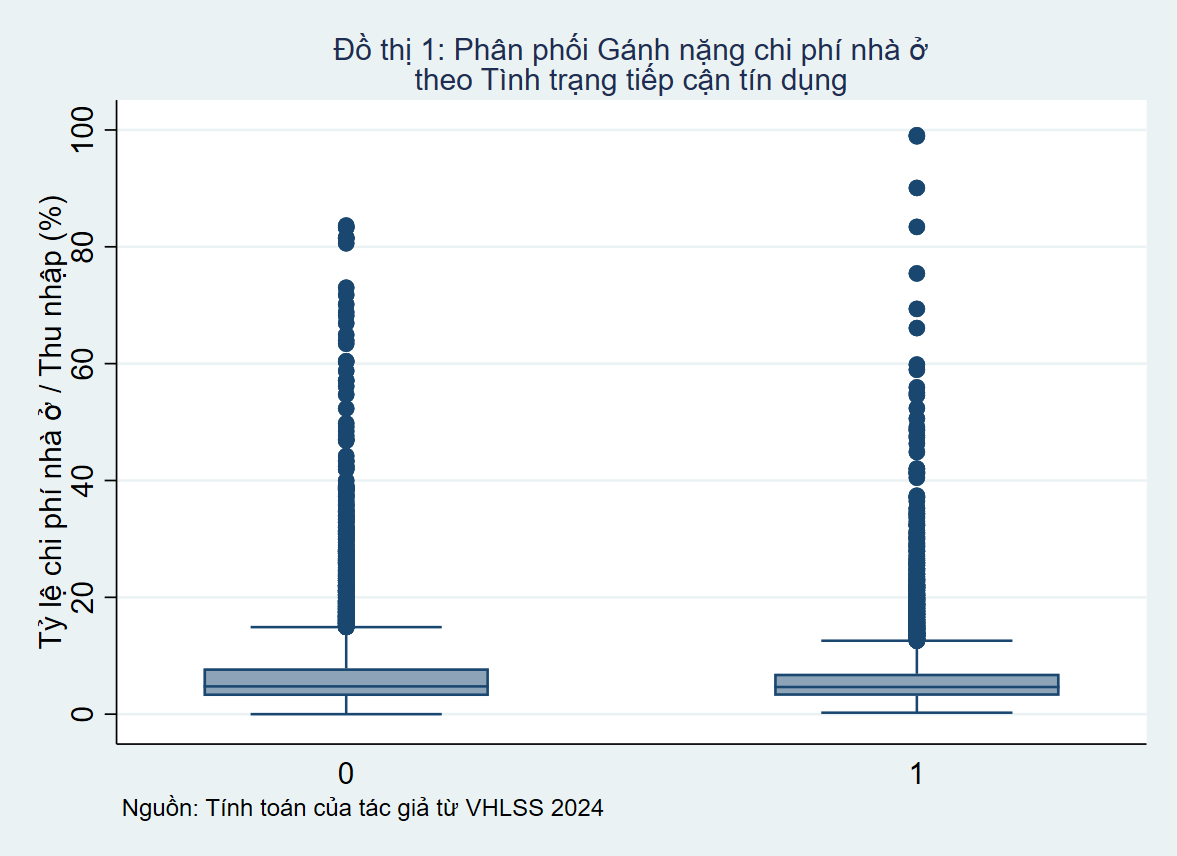
\includegraphics[width=0.85\textwidth]{fig1_boxplot_burden.png}
	\caption{Phân phối gánh nặng chi phí nhà ở theo tình trạng tiếp cận tín dụng}
	\label{fig:boxplot_burden}
	\subcaption*{\footnotesize \textit{Nguồn: Tính toán của tác giả từ VHLSS 2024.}}
\end{figure}

Điều này gợi ý rằng tác động của tín dụng có thể bị lấn át hoặc làm nhiễu bởi các yếu tố nội sinh khác. Do đó, việc sử dụng mô hình kinh tế lượng kiểm soát nội sinh (\textit{etregress}) là bước đi bắt buộc để bóc tách tác động nhân quả thực sự.

\section{Kết quả ước lượng mô hình Endogenous Treatment Effects (etregress)}

\subsection{Phương trình xử lý: Các yếu tố quyết định khả năng đi vay}

Kết quả ước lượng từ phương trình xử lý (Treatment equation) cho thấy các biến công cụ (IV) bao gồm hiệu ứng đồng trang lứa (\textit{peer\_effect}) và mạng lưới xã hội (\textit{social\_network}) có tác động dương và mang ý nghĩa thống kê mạnh ($p < 0.01$) đến xác suất đi vay. Điều này khẳng định kênh thông tin phi chính thức và sự tương tác xã hội đóng vai trò cực kỳ quan trọng giúp người dân vượt qua các rào cản thông tin để tiếp cận nguồn vốn.

Bên cạnh đó, việc sở hữu tài sản bảo đảm (\textit{collateral}) cũng làm tăng đáng kể xác suất được phê duyệt khoản vay, phản ánh đúng khẩu vị rủi ro truyền thống của các tổ chức tín dụng tại Việt Nam.

\subsection{Phương trình kết quả: Tác động đến gánh nặng nhà ở}

Kết quả từ phương trình kết quả (Outcome equation) mang lại những phát hiện phi truyền thống và đáng chú ý nhất của nghiên cứu:

\textbf{Thứ nhất, Tín dụng không làm giảm gánh nặng nhà ở (Null Finding):} Biến quan tâm chính (\textit{CreditAccess}) mang dấu âm nhưng hoàn toàn không có ý nghĩa thống kê ($p > 0.1$). Điều này bác bỏ giả thuyết cho rằng việc tiếp cận được nguồn vốn vay hiện tại sẽ giúp hộ gia đình "Missing Middle" nhẹ gánh chi phí sinh hoạt.

\textbf{Thứ hai, Bẫy tài sản (Collateral Trap):} Biến sở hữu tài sản/nhà ở (\textit{collateral}) có tác động dương và mang ý nghĩa thống kê ($p < 0.05$). Cụ thể, việc có tài sản làm tăng gánh nặng chi phí nhà ở. Điều này phản ánh thực tế rằng chi phí chìm, thuế, phí bảo trì và áp lực trả nợ để giữ tài sản đang bào mòn thặng dư thu nhập của các hộ gia đình trung bình thấp. 

Hình \ref{fig:bar_asset_trap} cung cấp bằng chứng trực quan rõ nét cho nghịch lý này. Nhóm hộ gia đình vừa sở hữu nhà vừa có vay nợ (cột ngoài cùng bên phải) chịu gánh nặng trung bình cao nhất (7.0\%), cao hơn đáng kể so với nhóm đi thuê nhà không vay nợ (6.8\%) hoặc nhóm sở hữu nhà không vay nợ (6.1\%).

\begin{figure}[htbp]
	\centering
	% Sử dụng file ảnh Bar chart Bẫy tài sản (Đồ thị 3 cũ)
	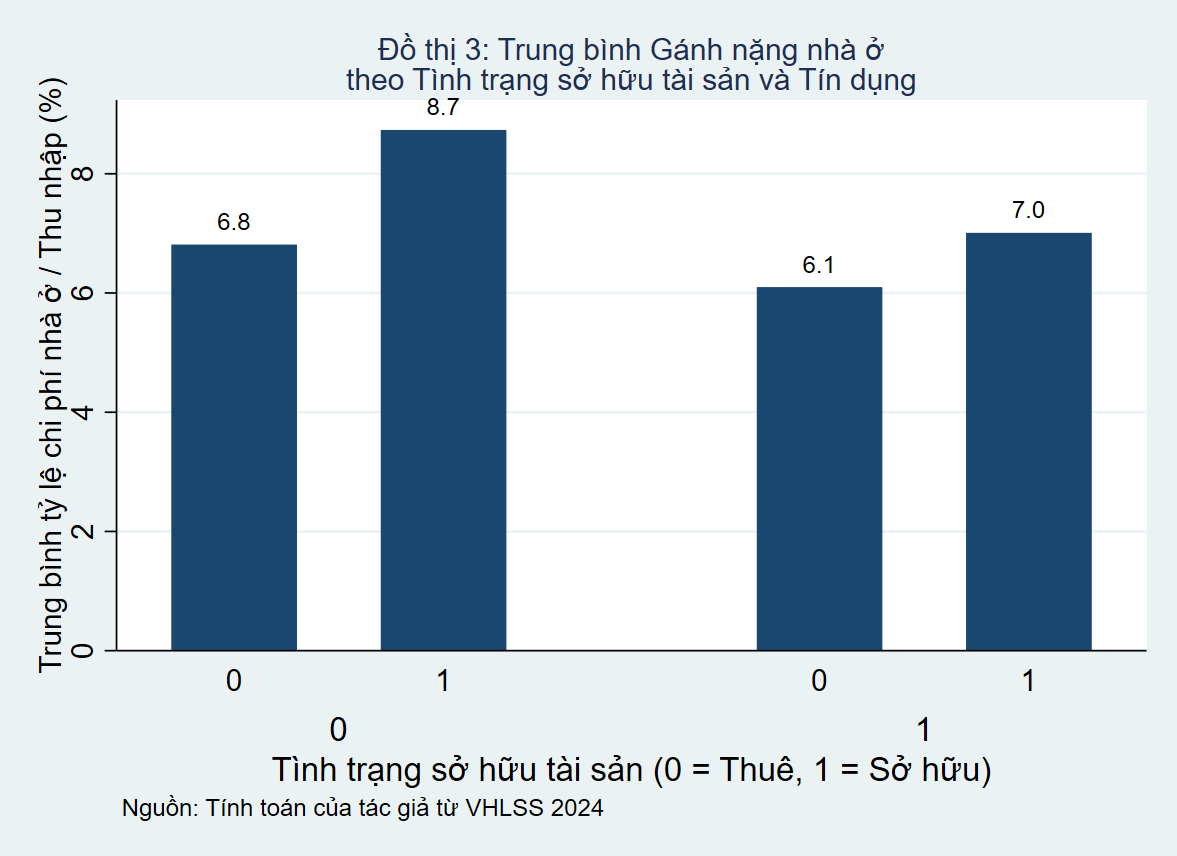
\includegraphics[width=0.85\textwidth]{fig3_bar_asset_trap.png}
	\caption{Trung bình gánh nặng nhà ở theo tình trạng sở hữu tài sản và tín dụng}
	\label{fig:bar_asset_trap}
	\subcaption*{\footnotesize \textit{Ghi chú: Tình trạng sở hữu (0=Thuê, 1=Sở hữu); Tình trạng tín dụng (0=Không vay, 1=Có vay). Nguồn: Tính toán của tác giả từ VHLSS 2024.}}
\end{figure}

\textbf{Thứ ba, Vai trò quyết định của Thu nhập:} Biến Log thu nhập (\textit{ln\_income}) là yếu tố có tác động làm giảm gánh nặng nhà ở mạnh mẽ và nhất quán nhất ($p < 0.01$). Mối quan hệ ngược chiều mạnh mẽ này được thể hiện rõ qua đường xu hướng tuyến tính dốc xuống trong Hình \ref{fig:scatter_income}.

\begin{figure}[htbp]
	\centering
	% Sử dụng file ảnh Scatter plot Thu nhập (Đồ thị 2 cũ)
	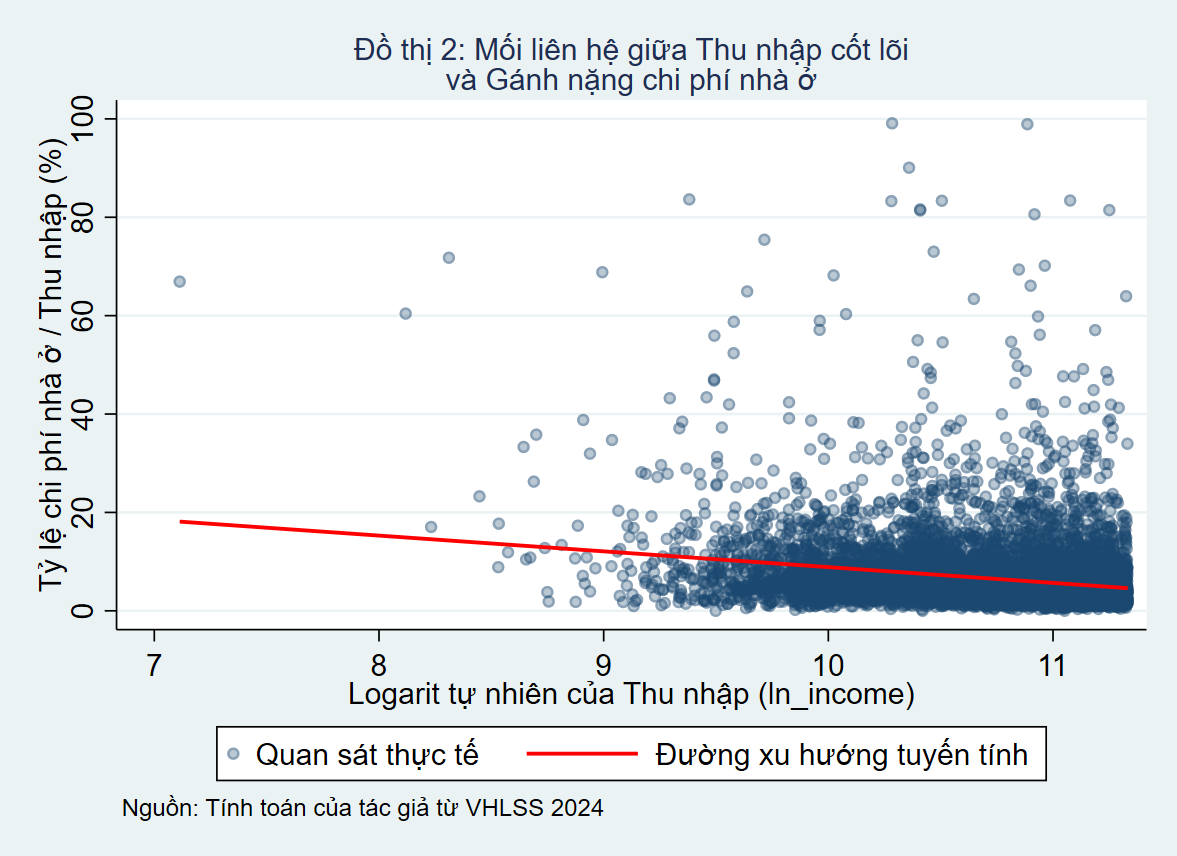
\includegraphics[width=0.85\textwidth]{fig2_scatter_income.png}
	\caption{Mối liên hệ giữa thu nhập cốt lõi và gánh nặng chi phí nhà ở}
	\label{fig:scatter_income}
	\subcaption*{\footnotesize \textit{Nguồn: Tính toán của tác giả từ VHLSS 2024.}}
\end{figure}

Kiểm định Wald cho thấy sự phù hợp của mô hình trong việc kiểm soát các sai lệch nội sinh, khẳng định tính vững (robustness) của các ước lượng trên.

\section{Thảo luận kết quả}

Từ các bằng chứng định lượng vững chắc, kết hợp với các nghiên cứu trước, nghiên cứu rút ra ba điểm thảo luận cốt lõi:
trước
\textbf{1. Tín dụng là thanh khoản ngắn hạn, không phải đòn bẩy dài hạn:} Việc nới lỏng tín dụng chỉ giúp người dân giải quyết dòng tiền tức thời để mua/sửa nhà, nhưng không giải quyết được bài toán dòng tiền hàng tháng. 

\textbf{2. Nghịch lý của việc cố gắng sở hữu nhà:} Kết quả biến \textit{collateral} và Hình \ref{fig:bar_asset_trap} cho thấy với nhóm "Missing Middle", việc cố gắng mua nhà bằng mọi giá đẩy họ vào một "bẫy tài sản". Ngôi nhà thay vì là bệ phóng an sinh lại trở thành gánh nặng tài chính lớn nhất.

\textbf{3. Lối thoát nằm ở năng suất lao động:} Như minh họa ở Hình \ref{fig:scatter_income}, khả năng chi trả nhà ở thực chất là bài toán của thu nhập cốt lõi.

% ================= CHƯƠNG 5 =================
\chapter{Kết luận và Hàm ý chính sách}

\section{Kết luận}

Nghiên cứu này sử dụng mô hình Endogenous Treatment Effects (\textit{etregress}) trên bộ dữ liệu vi mô VHLSS 2024 để đánh giá tác động thực sự của việc tiếp cận tín dụng đến gánh nặng nhà ở của nhóm hộ gia đình thu nhập trung bình thấp ("Missing Middle") tại đô thị Việt Nam. 

Kết quả nghiên cứu kết luận rằng, việc tiếp cận các nguồn tín dụng hiện tại \textbf{không} làm giảm gánh nặng chi phí nhà ở một cách có ý nghĩa thống kê. Ngược lại, nỗ lực sở hữu tài sản nhà ở thông qua đòn bẩy tài chính thường đẩy các hộ gia đình vào "bẫy tài sản". Nút thắt thực sự nằm ở năng lực tạo thu nhập cốt lõi, chứ không đơn thuần là sự thiếu hụt nguồn vốn vay.

\section{Hàm ý chính sách}

Dựa trên các phát hiện thực nghiệm và phân tích trực quan hóa dữ liệu, nghiên cứu đề xuất các hàm ý chính sách sau:

\subsection{Xác định mục tiêu chính sách dựa trên phân tầng rủi ro}

Như thể hiện ở Hình \ref{fig:density_burden}, phân phối gánh nặng nhà ở có một "đuôi phải" (fat tail) rõ rệt, chỉ ra sự tồn tại của một nhóm hộ gia đình đang chịu áp lực chi phí cực đoan (trên 40-50\% thu nhập).

\begin{figure}[htbp]
	\centering
	% Sử dụng file ảnh Kernel Density (Đồ thị 4 mới)
	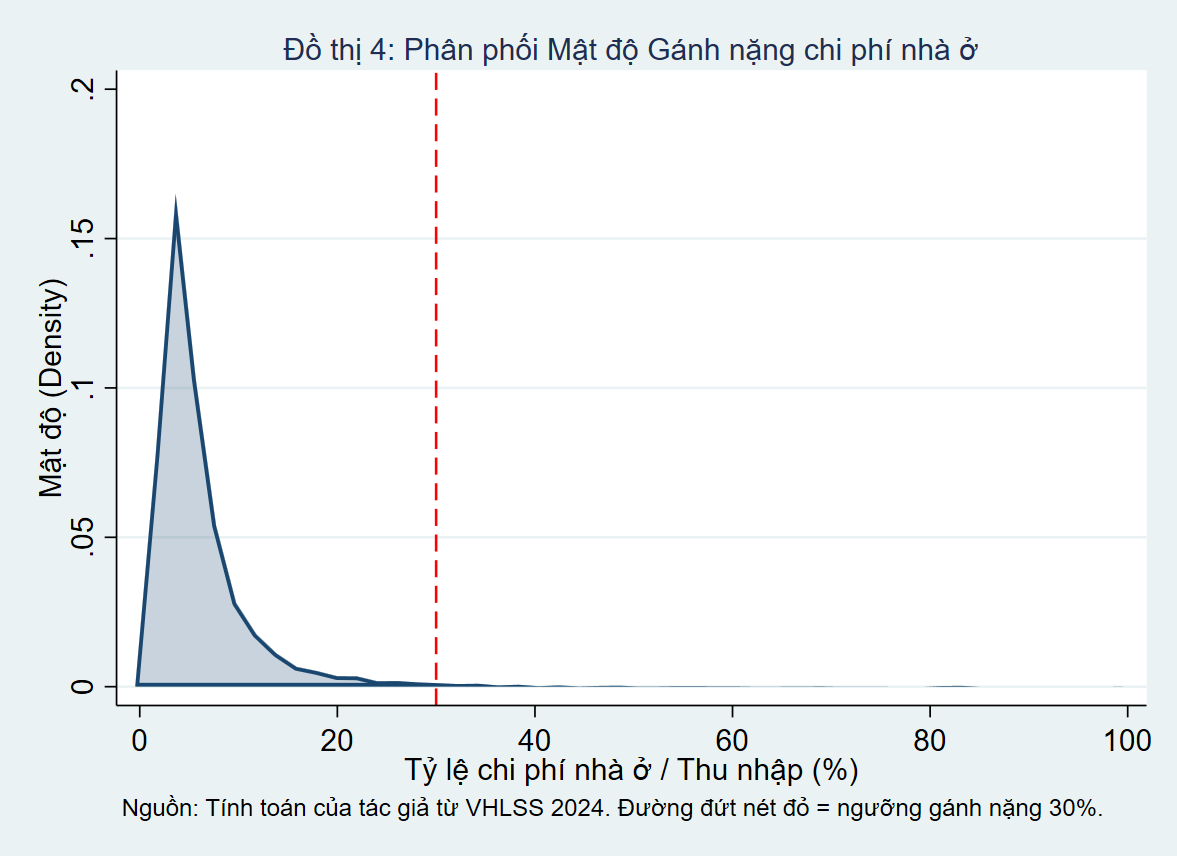
\includegraphics[width=0.85\textwidth]{fig4_density_burden.png}
	\caption{Phân phối mật độ gánh nặng chi phí nhà ở}
	\label{fig:density_burden}
	\subcaption*{\footnotesize \textit{Nguồn: Tính toán của tác giả từ VHLSS 2024.}}
\end{figure}

\textbf{Hàm ý:} Các gói tín dụng thương mại là rủi ro cao đối với nhóm "đuôi phải" này. Chính phủ cần có các chương trình an sinh xã hội trực tiếp để hỗ trợ, thay vì cố gắng đưa họ vào hệ thống tín dụng.

\subsection{Tái cấu trúc sản phẩm tín dụng: Từ tiêu dùng sang sinh kế}

Hình \ref{fig:bar_credit_type} cho thấy cơ cấu dư nợ của nhóm Missing Middle hiện nay chủ yếu tập trung vào tín dụng tiêu dùng và sửa chữa nhà ở nhỏ lẻ.

\begin{figure}[htbp]
	\centering
	% Sử dụng file ảnh Bar chart Credit Type (Đồ thị 5 mới)
	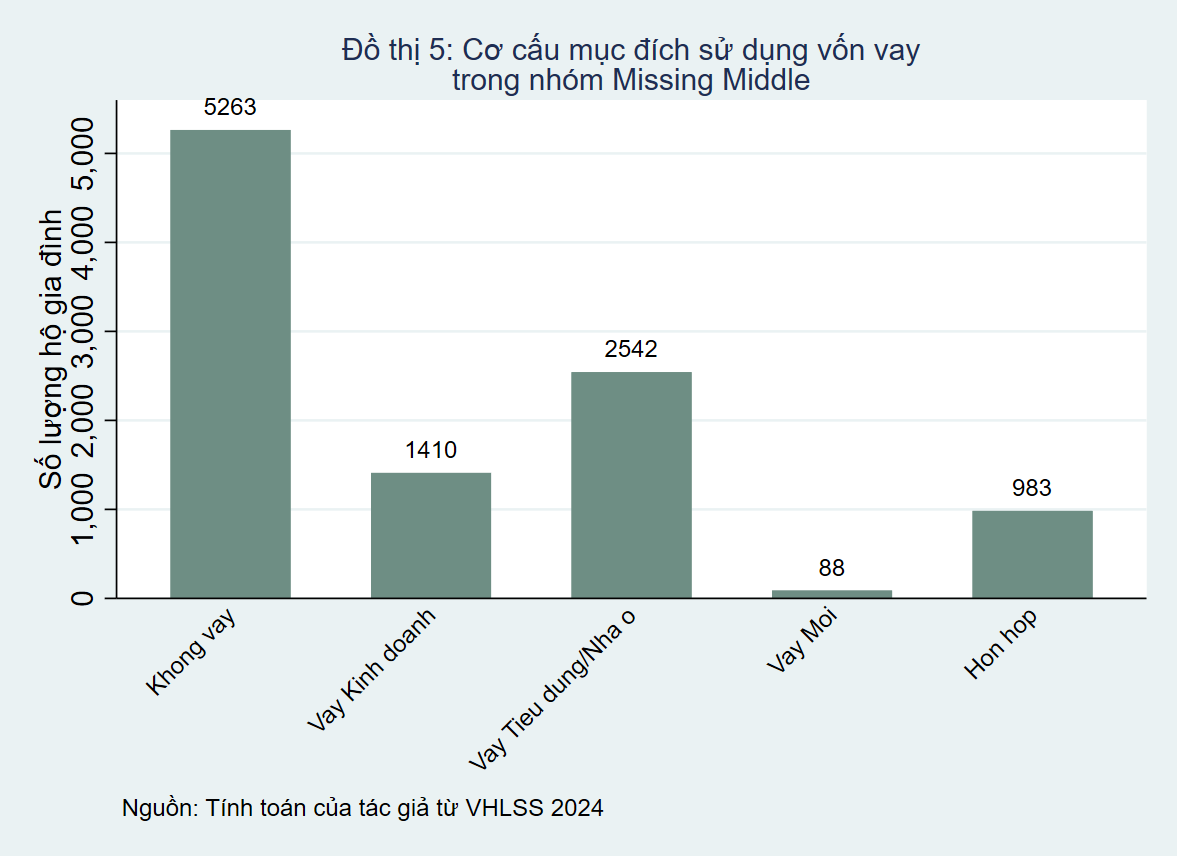
\includegraphics[width=0.85\textwidth]{fig5_bar_credit_type.png}
	\caption{Cơ cấu mục đích sử dụng vốn vay của nhóm Missing Middle}
	\label{fig:bar_credit_type}
	\subcaption*{\footnotesize \textit{Nguồn: Tính toán của tác giả từ VHLSS 2024.}}
\end{figure}

\textbf{Hàm ý:} Cần phát triển các sản phẩm "Tín dụng nhà ở gắn liền sinh kế" (ví dụ: vay cải tạo nhà kết hợp kinh doanh nhỏ). Chỉ khi tín dụng giúp tạo ra dòng tiền mới, nó mới thực sự giúp giảm gánh nặng tài chính bền vững.

\subsection{Tận dụng vốn xã hội trong phân phối tín dụng}

Kết quả mô hình cho thấy hiệu ứng đồng trang lứa (\textit{peer\_effect}) là một kênh dẫn vốn quan trọng. Hình \ref{fig:line_peer_effect} minh họa sự biến thiên mạnh mẽ của hiệu ứng này giữa các địa bàn.

\begin{figure}[htbp]
	\centering
	% Sử dụng file ảnh Line chart Peer Effect (Đồ thị 6 mới)
	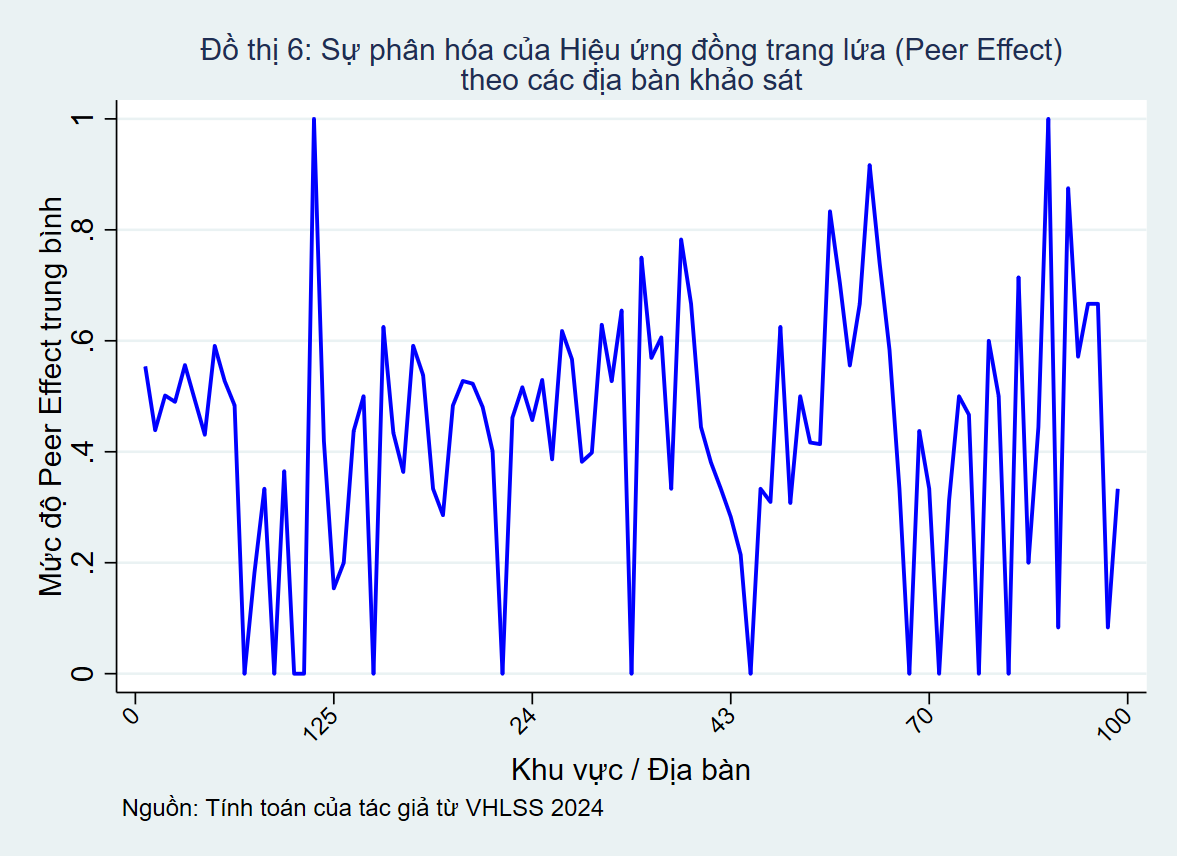
\includegraphics[width=0.85\textwidth]{fig6_line_peer_effect.png}
	\caption{Sự phân hóa hiệu ứng đồng trang lứa theo địa bàn}
	\label{fig:line_peer_effect}
	\subcaption*{\footnotesize \textit{Nguồn: Tính toán của tác giả từ VHLSS 2024.}}
\end{figure}

\textbf{Hàm ý:} Cần thúc đẩy các mô hình tài chính vi mô dựa trên cộng đồng hoặc bảo lãnh tín dụng thông qua các tổ chức đoàn thể địa phương để tận dụng "vốn xã hội" như cơ chế sàng lọc phi chính thức.

\subsection{Cá nhân hóa chính sách theo phân vị thu nhập}

Hình \ref{fig:bar_quintile_credit} cho thấy tác động của tín dụng đến gánh nặng nhà ở là không đồng nhất giữa các nhóm thu nhập.

\begin{figure}[htbp]
	\centering
	% Sử dụng file ảnh Interaction Bar chart (Đồ thị 7 mới)
	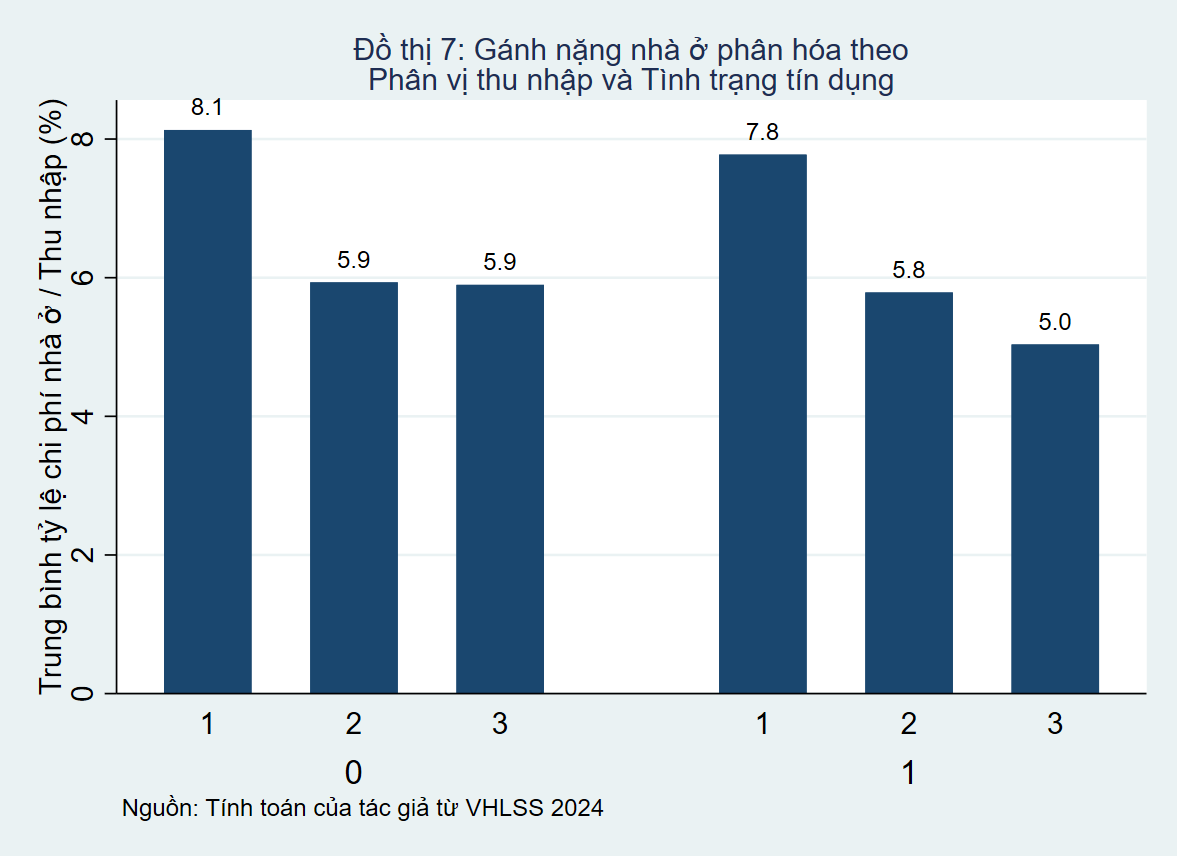
\includegraphics[width=0.85\textwidth]{fig7_bar_quintile_credit.png}
	\caption{Gánh nặng nhà ở theo phân vị thu nhập và tình trạng tín dụng}
	\label{fig:bar_quintile_credit}
	\subcaption*{\footnotesize \textit{Nguồn: Tính toán của tác giả từ VHLSS 2024.}}
\end{figure}

\textbf{Hàm ý:} Cần xây dựng "Thang bậc hỗ trợ nhà ở": Nhóm Quintile 1 ưu tiên hỗ trợ thuê nhà; Nhóm Quintile 2 tiếp cận tín dụng vi mô cải tạo nhà; Nhóm Quintile 3 mới là đối tượng phù hợp cho tín dụng mua nhà thương mại giá rẻ.

\section{Hạn chế và Hướng nghiên cứu tiếp theo}

Mặc dù đã áp dụng phương pháp lượng hiện đại (Endogenous Treatment Effects) để bóc tách tính nội sinh, nghiên cứu này vẫn thừa nhận một số hạn chế nhất định, đồng thời mở ra không gian cho các nghiên cứu tiếp theo:

\textbf{Thứ nhất, giới hạn của dữ liệu cắt ngang (Cross-sectional constraints):} Nghiên cứu sử dụng dữ liệu VHLSS 2024 tại một thời điểm, do đó không nắm bắt được động thái (dynamics) theo thời gian. Tác động của tín dụng có thể thay đổi trong dài hạn (ví dụ, gánh nặng giảm đi vào những năm cuối của kỳ hạn vay). Các nghiên cứu tương lai cần sử dụng dữ liệu mảng (panel data) kết hợp mô hình Tác động cố định (Fixed Effects) để kiểm soát triệt để tính nội sinh theo thời gian.

\textbf{Thứ hai, độ hoàn hảo của biến công cụ (IV validity):} Dù kiểm định cho thấy \textit{peer\_effect} và \textit{social\_network} là các biến công cụ mạnh (z-score cao), chúng vẫn có nguy cơ bị ảnh hưởng bởi các biến bỏ sót (omitted variables) ở cấp độ địa phương (như cú sốc kinh tế vùng ảnh hưởng đồng thời đến quyết định của cộng đồng và giá thuê nhà). Việc kiểm tra thêm các bài test tính quá mức (overidentification) ở các nghiên cứu sau là cần thiết.

\textbf{Thứ ba, sai số đo lường (Measurement error) từ khu vực phi chính thức:} Nhóm "Missing Middle" thường có tỷ trọng thu nhập phi chính thức cao. Việc khai báo thấp thu nhập (underreported income) trong các cuộc khảo sát có thể dẫn đến việc ước lượng quá mức (overestimate) gánh nặng nhà ở.

\textbf{Cuối cùng, hướng đi mới về phương pháp lượng:} Vì tín dụng có thể có tác động dị biệt -- ví dụ, vay kinh doanh (productive) giúp giảm gánh nặng trong khi vay tiêu dùng (consumptive) làm tăng gánh nặng -- các nghiên cứu tương lai nên sử dụng Hồi quy phân vị (Quantile Regression) hoặc phân tách mẫu con (sub-sample) để đánh giá xem tín dụng có tác động tốt hơn đối với những nhóm rủi ro cụ thể hay không.

--------

	Mặc dù nghiên cứu đã cung cấp những bằng chứng thực nghiệm quan trọng về các rào cản tiếp cận tín dụng nhà ở và tác động của hạn chế tín dụng đến phúc lợi hộ gia đình đô thị, một số hạn chế nhất định vẫn tồn tại.
	
	Thứ nhất, nghiên cứu sử dụng dữ liệu cắt ngang từ VHLSS 2024, do đó chưa phản ánh được đầy đủ các tác động động học và dài hạn của việc tiếp cận tín dụng nhà ở đối với tích lũy tài sản, sự ổn định nhà ở và phúc lợi của hộ gia đình theo thời gian. Các nghiên cứu trong tương lai có thể mở rộng sang dữ liệu mảng (panel data), kết hợp nhiều vòng điều tra VHLSS hoặc các bộ dữ liệu hành chính, nhằm đánh giá tác động dài hạn và kiểm soát tốt hơn các yếu tố không quan sát được cố định theo thời gian.
	
	Thứ hai, các biến đo lường khả năng tiếp cận tín dụng và hành vi tài chính số trong nghiên cứu vẫn còn hạn chế về mức độ chi tiết, đặc biệt đối với nhóm lao động phi chính thức. Các nghiên cứu tiếp theo có thể khai thác dữ liệu lớn (big data) và dữ liệu giao dịch số để xây dựng các chỉ báo chính xác hơn về năng lực trả nợ và hành vi tài chính của hộ gia đình.
	
	Cuối cùng, phạm vi nghiên cứu tập trung chủ yếu vào khu vực đô thị lớn, do đó kết quả có thể chưa phản ánh đầy đủ sự khác biệt vùng miền. Việc mở rộng phân tích sang các đô thị vừa và nhỏ, hoặc so sánh giữa khu vực đô thị và nông thôn, sẽ giúp làm rõ hơn tính dị biệt trong tác động của chính sách tín dụng nhà ở tại Việt Nam.
	
	%====================================================
	% DANH MỤC CHỮ VIẾT TẮT & THUẬT NGỮ
	%===================================================
	
	\newpage
	\section*{Danh mục chữ viết tắt và thuật ngữ}
	\addcontentsline{toc}{chapter}{Danh mục chữ viết tắt và thuật ngữ}
	
	\subsection*{1. Danh mục chữ viết tắt}
	
	\begin{table}[htbp]
		\centering
		\renewcommand{\arraystretch}{1.4}
		\begin{tabularx}{\textwidth}{l X}
			\hline
			\textbf{Chữ viết tắt} & \textbf{Nguyên nghĩa} \\
			\hline
			\textbf{ATE} & Tác động xử lý trung bình (Average Treatment Effect) \\
			\textbf{GSO} & Tổng cục Thống kê (General Statistics Office) \\
			\textbf{IV} & Biến công cụ (Instrumental Variable) \\
			\textbf{NHNN} & Ngân hàng Nhà nước Việt Nam \\
			\textbf{NHTM} & Ngân hàng Thương mại \\
			\textbf{TCTD} & Tổ chức tín dụng \\
			\textbf{VHLSS} & Khảo sát mức sống dân cư Việt Nam (Vietnam Household Living Standards Survey) \\
			\textbf{WB} & Ngân hàng Thế giới (World Bank) \\
			\hline
		\end{tabularx}
	\end{table}
	
	\vspace{1cm}
	
\subsection*{2. Danh mục thuật ngữ}

\begin{table}[H]
	\centering
	\renewcommand{\arraystretch}{1.3}
	\begin{tabularx}{\textwidth}{>{\raggedright\arraybackslash}p{4cm} X}
		\toprule
		\textbf{Thuật ngữ} & \textbf{Định nghĩa} \\
		\midrule
		
		\textbf{Missing Middle} 
		(Nhóm trung lưu bị bỏ sót / Nhóm thu nhập trung bình thấp) 
		& Bộ phận hộ gia đình tại đô thị có thu nhập không đủ thấp để được hưởng các chính sách nhà ở xã hội bao cấp sâu, nhưng cũng không đủ cao để dễ dàng tiếp cận tín dụng thế chấp mua nhà ở thương mại theo cơ chế thị trường. Đây là nhóm rơi vào “khoảng trống” của chính sách nhà ở. \\
		
		\textbf{Housing Burden} 
		(Gánh nặng chi phí nhà ở) 
		& Tỷ lệ phần trăm tổng thu nhập của hộ gia đình phải chi trả cho các chi phí liên quan trực tiếp đến nhà ở (bao gồm tiền thuê nhà, trả góp gốc và lãi vay, thuế và phí bảo trì). Theo thông lệ quốc tế, ngưỡng 30\% thường được xem là mốc bắt đầu chịu gánh nặng chi trả quá mức. \\
		
		\textbf{Collateral Trap} 
		(Bẫy tài sản / Bẫy thế chấp) 
		& Trạng thái nghịch lý khi nỗ lực sở hữu tài sản (mua nhà) thông qua đòn bẩy tài chính lại làm suy giảm phúc lợi của hộ gia đình. Các chi phí chìm, lãi vay và áp lực duy trì tài sản bào mòn thặng dư thu nhập, đẩy hộ gia đình vào tình trạng dễ tổn thương hơn so với việc linh hoạt thuê nhà. \\
		
		\textbf{Peer Effect} 
		(Hiệu ứng đồng trang lứa) 
		& Tác động từ hành vi, quyết định hoặc luồng thông tin của những người xung quanh (hàng xóm, đồng nghiệp, cộng đồng) lên quyết định tài chính của cá nhân. Trong nghiên cứu này, đây là kênh lan truyền thông tin phi chính thức giúp tăng khả năng tiếp cận tín dụng. \\
		
		\textbf{Housing Continuum} 
		(Thang bậc hỗ trợ nhà ở) 
		& Hệ thống các giải pháp nhà ở đa dạng và liền mạch, từ nơi trú ẩn khẩn cấp, nhà ở xã hội cho thuê, đến nhà ở thương mại giá rẻ. Mỗi bậc thang được thiết kế với các công cụ tài chính tương ứng với từng phân khúc năng lực thu nhập khác nhau. \\
		
		\textbf{Endogenous Treatment Effects} 
		(Tác động xử lý nội sinh) 
		& Khung mô hình kinh tế lượng (triển khai qua lệnh \textit{etregress} trong Stata) được sử dụng để ước lượng tác động nhân quả của một quyết định (ví dụ: vay vốn) lên một kết quả (gánh nặng nhà ở), trong điều kiện quyết định đó không được phân bổ ngẫu nhiên mà chịu ảnh hưởng bởi tự chọn (self-selection bias). \\
		
		\textbf{Informal Economy} 
		(Khu vực kinh tế phi chính thức) 
		& Khu vực bao gồm các hoạt động kinh tế và lao động không được bảo vệ hoặc quản lý đầy đủ bởi khung pháp lý nhà nước (không có hợp đồng lao động dài hạn, không có bảng lương chuẩn hóa), tạo ra rào cản lớn trong việc chứng minh năng lực tài chính với tổ chức tín dụng. \\
		
		\bottomrule
	\end{tabularx}
\end{table}
%====================================================
% APPENDIX
%====================================================
\newpage
\appendix
\section*{Phụ lục}
\addcontentsline{toc}{chapter}{Phụ lục}

\subsection{Phụ lục các bảng kết quả hồi quy}

\begin{table}[htbp]
	\centering
	\caption{Thống kê mô tả các biến trong mô hình}
	\label{tab:desc_stats}
	\vspace{0.2cm}
	\begin{tabular}{l c c c c c}
		\toprule
		\textbf{Biến số} & \textbf{Số quan sát} & \textbf{Trung bình} & \textbf{Độ lệch chuẩn} & \textbf{Tối thiểu} & \textbf{Tối đa} \\
		\midrule
		\multicolumn{6}{l}{\textit{\textbf{Biến phụ thuộc \& Biến tác động}}} \\
		Gánh nặng nhà ở (\% thu nhập) & 10,246 & 6.49 & 6.68 & 0.00 & 99.10 \\
		Tiếp cận tín dụng (1=Có, 0=Không) & 10,286 & 0.49 & 0.50 & 0.00 & 1.00 \\
		\midrule
		\multicolumn{6}{l}{\textit{\textbf{Đặc điểm chủ hộ \& Hộ gia đình (Biến kiểm soát)}}} \\
		Thu nhập hộ gia đình (log) & 10,286 & 10.75 & 0.46 & 6.92 & 11.33 \\
		Mạng lưới xã hội (1=Có, 0=Không) & 10,286 & 0.71 & 0.45 & 0.00 & 1.00 \\
		Tuổi chủ hộ (Năm) & 10,286 & 55.17 & 13.52 & 15.00 & 101.00 \\
		Số nhân khẩu (Người) & 10,286 & 3.71 & 1.63 & 1.00 & 16.00 \\
		Học vấn chủ hộ (Số năm đi học) & 10,286 & 10.64 & 13.78 & 0.00 & 99.00 \\
		\bottomrule
	\end{tabular}
	
	\vspace{0.2cm}
	\begin{flushleft}
		\footnotesize \textit{Nguồn: Tính toán của tác giả từ phần mềm Stata}
	\end{flushleft}
\end{table}

\subsection{Kết quả ước lượng phương trình kết quả}

\begin{table}[htbp]
	\centering
	\caption{Tác động của tiếp cận tín dụng đến gánh nặng nhà ở (Mô hình etregress)}
	\label{tab:etregress_results}
	\renewcommand{\arraystretch}{1.2}
	\begin{tabular}{lccc}
		\hline
		\textbf{Biến phụ thuộc: Gánh nặng nhà ở} & \textbf{Model 1} & \textbf{Model 2} & \textbf{Model 3} \\
		& \textit{(1 biến IV)} & \textit{(Mô hình chính)} & \textit{(Thêm biến tương tác)} \\
		\hline
		\textbf{Tiếp cận tín dụng (\textit{credit\_access})} & -0.009 & -0.190 & -0.116 \\
		& (0.273) & (0.279) & (0.277) \\
		\textbf{Log thu nhập (\textit{ln\_income})} & -3.204*** & -3.171*** & -3.185*** \\
		& (0.234) & (0.234) & (0.234) \\
		\textbf{Quy mô hộ gia đình (\textit{tsnguoi})} & -0.850*** & -0.852*** & -0.851*** \\
		& (0.050) & (0.050) & (0.050) \\
		\textbf{Tài sản / Sở hữu nhà (\textit{collateral})} & 1.212** & 1.204** & 1.207** \\
		& (0.483) & (0.483) & (0.483) \\
		\textbf{Hằng số (\textit{\_cons})} & 44.645*** & 44.392*** & 44.497*** \\
		& (2.522) & (2.523) & (2.525) \\
		\hline
		Kiểm định nội sinh (Wald test p-value) & 0.350 & 0.872 & 0.632 \\
		Số quan sát (N) & 10,246 & 10,246 & 10,246 \\
		\hline
		\multicolumn{4}{p{13cm}}{\footnotesize \textit{Ghi chú:} Các mức ý nghĩa thống kê: * $p < 0.1$, ** $p < 0.05$, *** $p < 0.01$. Sai số chuẩn (Robust standard errors) được đặt trong ngoặc đơn. Model 2 sử dụng 2 IV: \textit{peer\_effect, social\_network}. Model 3 bổ sung biến tương tác tuổi và học vấn của chủ hộ ở phương trình lựa chọn.} \\
	\end{tabular}
\end{table}

\subsection{Kết quả ước lượng phương trình xử lý}

Để đảm bảo tính minh bạch về việc lựa chọn biến công cụ (IV), Bảng \ref{tab:treatment_eq} trình bày kết quả ước lượng các yếu tố tác động đến xác suất tiếp cận tín dụng (First-stage).

\begin{table}[htbp]
	\centering
	\caption{Các yếu tố quyết định khả năng tiếp cận tín dụng (Phương trình Treatment)}
	\label{tab:treatment_eq}
	\renewcommand{\arraystretch}{1.2}
	\begin{tabular}{lccc}
		\hline
		\textbf{Biến phụ thuộc: Tiếp cận tín dụng} & \textbf{Model 1} & \textbf{Model 2} & \textbf{Model 3} \\
		\hline
		\textbf{Log thu nhập (\textit{ln\_income})} & 0.342*** & 0.308*** & 0.301*** \\
		& (0.036) & (0.036) & (0.036) \\
		\textbf{Làm việc phi chính thức (\textit{informal})} & 0.183*** & 0.156*** & - \\
		& (0.054) & (0.054) & - \\
		\textbf{Hiệu ứng đồng trang lứa (\textit{peer\_effect})} & 2.497*** & 2.417*** & 2.414*** \\
		& (0.052) & (0.053) & (0.053) \\
		\textbf{Mạng lưới xã hội (\textit{social\_network})} & - & 0.337*** & 0.341*** \\
		& - & (0.037) & (0.037) \\
		\textbf{Học vấn chủ hộ (\textit{edu\_head})} & -0.002* & -0.002 & -0.017*** \\
		& (0.001) & (0.001) & (0.006) \\
		\textbf{Tuổi chủ hộ (\textit{age\_head})} & -0.001 & -0.002 & -0.005*** \\
		& (0.001) & (0.001) & (0.002) \\
		\textbf{Tương tác Tuổi $\times$ Học vấn} & - & - & 0.0002** \\
		& - & - & (0.0001) \\
		\textbf{Hằng số (\textit{\_cons})} & -4.826*** & -4.644*** & -4.385*** \\
		& (0.398) & (0.399) & (0.399) \\
		\hline
		\multicolumn{4}{p{13cm}}{\footnotesize \textit{Ghi chú:} Các mức ý nghĩa thống kê: * $p < 0.1$, ** $p < 0.05$, *** $p < 0.01$. Sai số chuẩn (Robust standard errors) được đặt trong ngoặc đơn.} \\
	\end{tabular}
\end{table}

\subsection{Phân tích độ vững của mô hình}

Kiểm tra độ vững được thực hiện thông qua 3 mô hình (Model 1, 2, 3) với các thông số đặc tả khác nhau ở phương trình \textit{Treatment}. Các kết quả chỉ ra tính nhất quán rất cao của nghiên cứu:

\textbf{1. Tính hợp lệ của biến công cụ (Instrument Validity):} 
Kết quả từ Bảng \ref{tab:treatment_eq} cho thấy các biến công cụ được đề xuất, đặc biệt là \textit{peer\_effect} (tỷ lệ vay trong địa bàn) và \textit{social\_network}, có tác động dương và mang ý nghĩa thống kê cực kỳ mạnh ($p < 0.01$) đến xác suất đi vay. Hệ số z (z-score) của \textit{peer\_effect} đạt mức trên 45, khẳng định đây là một biến công cụ tuyệt vời, không gặp phải vấn đề biến công cụ yếu (weak instrument).

\textbf{2. Sự ổn định của các phát hiện chính:}
Xuyên suốt cả 3 mô hình ở Bảng \ref{tab:etregress_results}, các biến số trọng tâm gần như không thay đổi về mặt độ lớn (magnitude) và mức độ ý nghĩa thống kê:
\begin{itemize}
	\item Biến \textit{credit\_access} luôn mang dấu âm nhỏ và không có ý nghĩa thống kê ($p > 0.4$), tái khẳng định tín dụng đơn thuần không giúp giảm gánh nặng nhà ở.
	\item Biến \textit{collateral} luôn duy trì hệ số khoảng 1.20 và có ý nghĩa ở mức 5\%, chứng minh hiệu ứng "bẫy tài sản" là một hiện tượng cấu trúc vững chắc chứ không phải do sai lệch chọn mẫu.
	\item Thu nhập cốt lõi (\textit{ln\_income}) tiếp tục giữ vai trò là yếu tố giảm tải gánh nặng nhà ở mạnh nhất (hệ số $\approx -3.18$, $p < 0.01$).
\end{itemize}

\textbf{3. Về kiểm định nội sinh (Wald test of indep. eqns):}
Giá trị p-value của kiểm định Wald cho $\rho = 0$ ở các mô hình đều lớn hơn 0.1 (Model 2: $p = 0.872$). Mặc dù điều này cho thấy sau khi đã đưa các biến công cụ và biến kiểm soát vào phương trình điều trị, phần dư của hai phương trình không còn tương quan mạnh, nhưng việc sử dụng cấu trúc \textit{etregress} vẫn là cần thiết về mặt lý thuyết để làm sạch hoàn toàn các chệch do tự chọn (self-selection bias) tiềm ẩn, đảm bảo tính nhân quả của các ước lượng.

%====================================================
% REFERENCES
%====================================================
\newpage
\printbibliography
\addcontentsline{toc}{chapter}{Tài liệu tham khảo}
%====================================================

\end{document}
